\documentclass[useAMS,usenatbib]{mn2e}

%%%%% AUTHORS - PLACE YOUR OWN MACROS HERE %%%%%
\usepackage{graphicx}
\usepackage{amsmath}
\usepackage{graphicx}
\usepackage[T1]{fontenc}
\usepackage[utf8]{inputenc}

\newcommand{\aaps}{A\&AS}
\newcommand{\aap}{A\&A}
\newcommand{\mnras}{MNRAS}
\newcommand{\nat}{Nature}
\newcommand{\physrep}{Phys. Rep.}

\newcommand{\ee}{\mathrm{e}}
\newcommand{\ii}{\mathrm{i}}

%%% for our internal comments, use color
\usepackage[usenames,dvipsnames,svgnames,table]{xcolor}
\newcommand{\OMS}[1]{\textcolor{red}{{\bf OMS: #1}}}
\newcommand{\ATM}[1]{\textcolor{red}{{\bf Marcellin: #1}}}

%%%%%%%%%%%%%%%%%%%%%%%%%%%%%%%%%%%%%%%%%%%%%%%%

\title[BDWFs for data compression and FoV shaping]{Using baseline-dependent windowing functions 
for data compression and field-of-view shaping in radio interferometry}
\author[M.T. Atemkeng , O.M. Smirnov, C. Tasse, G. Foster and J. Jonas]{M.T. 
Atemkeng$^{1}$\thanks{E-mail: m.atemkeng@gmail.com}, O.M. Smirnov$^{12}$, C. Tasse$^{31}$, G. Foster$^{12}$, J. Jonas$^{12}$ \\
$^1$Department of Physics and Electronics, Rhodes University, PO Box 94, Grahamstown, 6140, South Africa\\
$^2$SKA South Africa, 3rd Floor, The Park, Park Road, Pinelands, 7405, South Africa\\
$^3$GEPI, Observatoire de Paris, CNRS, Universite Paris Diderot, 5 place Jules Janssen, 92190 Meudon, France}
\begin{document}

\date{in original form 2015 Sep 14}

\pagerange{\pageref{firstpage}--\pageref{lastpage}} \pubyear{2013}

\maketitle

\label{firstpage}

\begin{abstract}
This paper investigates the use of baseline-dependent windowing functions in radio interferometry. 

in order to reduce
the loss of amplitude (also known as smearing) when the correlated data is averaged over wide bandwidth and long 
integration times. 

In radio interferometry smearing is 
reduced when a cross-correlator averages the correlated data over narrower bandwidth and shorter integration times. Unfortunately, this 
leads to a huge amount of data to manage and it is becoming a bottleneck for further data processing such as calibration and 
imaging.  With future generation surveys, it is important to investigate the reduction of the output data rate. Therefore, the focus of 
this paper is on the use of baselines dependent windowing functions to keep smearing down at an acceptable extent and at the same time 
significantly suppress signals 
from out field of view sources, while the nominal sensitivity is conserved. 
\end{abstract}
\begin{keywords}
Instrumentation: interferometers, Methods: data analysis, Methods: numerical, Techniques: interferometric
\end{keywords}

\section[]{Introduction}

A radio interferometer measures complex quantities called \emph{visibilities}, which, following the van Cittert-Zernike 
relation \citep{thompson1999fundamentals,thompson2001fundamentals}, correspond to Fourier modes of the sky brightness distribution, corrupted by various instrumental 
and atmospheric effects. One particular effect, known as \emph{time} and \emph{bandwidth smearing} (or averaging) occurs 
when the visibilities are averaged over a time and frequency bin of non-zero extent \citep{bridle1989wide,bridle1999bandwidth}. This unavoidably happens in the correlator 
(since the correlator output is, by definition, an average measurement over some interval), but also if data is further 
averaged post-correlation (both for purposes of compression, and to reduce computational cost).

The effect of smearing is mainly a decrease in the amplitude of off-axis sources. This is easy to understand: the visibility contribution of a point source of flux $S$ located in the direction given by the unit vector $\bmath{\sigma}$ is given by

\begin{equation}
V = S \exp \big \{  \frac{2\pi i}{\lambda} \bmath{u}\cdot(\bmath{\sigma}-\bmath{\sigma}_0) \big \},
\end{equation}

where $\bmath{u}$ is the baseline vector, and $\bmath{\sigma}_0$ is the phase centre (or fringe stopping centre) of the observation.
The complex phase term above rotates as a function of frequency (due to the inverse scaling with $\lambda$) and time (due to
the fact that $\bmath{u}$ changes with time, at least in an Earth- or orbit-based interferometer). 
Taking a vector average over a time/frequency bin then results  in a net loss of amplitude. The effect increases 
with baseline length and distance from phase centre. Besides reducing apparent source flux, smearing also distorts the PSF, since different baselines (and thus different Fourier modes) are attenuated differently.

In the era of big interferometers, where computation (and thus data size) becomes one of the main cost drivers, it is 
in principle desirable to average the data down as much as possible, without compromising the science goals. There are natural limits to this: firstly, we still need to critically sample the $uv$-plane, secondly, we need to retain sufficient spectral resolution, thirdly, we don't want to average (at least pre-calibration) beyond the natural variation of the calibration parameters, and fourthly, we want to keep smearing at acceptable levels in order not to lose too much signal. In this work, we concentrate specifically on the smearing problem. Here, we can identify two regimes:

\begin{itemize}
\item In a compact interferometer, the maximum usable field of view (FoV) corresponds to the primary beam (PB) of the antennas; in
most cases (but surveys especially) we want the effective FoV to reach this limit. This imposes an upper limit on the size of a 
time/frequency bin: it must be small enough to keep amplitude loss acceptably low across the entire PB FoV. 
\item In VLBI, smearing is a lot more severe, so the effective FoV is determined by the smallest time/frequency bin size that a
correlator can support, and is normally much smaller than the PB. Modern VLBI correlators overcome this by employing a technique 
called multiple phase centre correlation, where the signal is correlated relative to multiple phase centres simultaneously, thus
effectively ``tiling'' the PB by multiple FoVs. This has a computational cost that scales linearly with the number of phase centres.
\end{itemize}

On the other hand, smearing also has a useful side effect. In interferometry, anything outside the desired FoV is unwanted 
signal. However, the PB pattern of any real-life antenna features sidelobes and backlobes 
that extend across the entire sky, albeit at a relatively faint level. The faintness makes sidelobes useless for imaging any 
but the brightest sources: the scientifically usable FoV is that given by the main lobe. However, the 
sum total signal from all the sources in the PB sidelobes, modulated by their PSF sidelobes, contributes an unwanted global 
background called the \emph{far sidelobe confusion noise} (FSCN). This imposes a fundamental sensitivity limit; in older 
telescopes and surveys this was well below the achievable thermal noise and therefore not a worry, but modern and future 
observatories are capable of reaching this limit \ATM{Please I could not find this reference or paper}\citep{Smirnov-FSCN}.
Even in observations well above the FSCN, individual extremely bright radio sources such as Cyg A or Cas A can contribute confusing signal from even the most distant 
sidelobe: the LOFAR telescope  \ATM{I am not so sure of this reference}\citep{LOFAR,tasse2013applying} has to deal with the so-called ``A-team'' sources on a routine basis. Since 
smearing suppresses distant sources, this somewhat alleviates both the FSCN and A-team problems.

When considering a short sequence of visibilities measured by one baseline, we can think of averaging as a convolution of the 
true visibility by a boxcar function corresponding to the $uv$-extent of the averaging bin, followed by sampling at the 
centre of each bin. Convolution in the visibility plane corresponds to multiplication of the image by a \emph{tapering function} 
that is the Fourier transform (FT) of the convolution kernel; the FT of a boxcar is a Sinc-type taper. If
we consider the entire $uv$-plane, averaging is only a pseudo-convolution, since the different $uv$-bins (and thus
their boxcars) will have different sizes and shapes as determined by baseline length and orientation. Still, we can 
qualitatively view smearing  as some kind of cumulative effect of an ensemble of image-plane tapers corresponding to all the 
different boxcars\footnote{For completeness, we should note that  this ``smearing taper'' is not the only tapering effect 
at work in interferometric imaging. Firstly, antennas have a non-zero 
physical extent: a measured visibility is already convolved by the aperture illumination functions (AIFs) of each pair of 
antennas. The resulting image-plane taper is exactly what the PB is. Secondly, most imaging software employs 
convolutional gridding followed by an FFT, which produces an additional taper that suppresses aliasing of sources from 
outside the imaged region.}. 

What if we were to employ weighted averaging instead of simple averaging (whether in the correlator, or in post-processing)? 
This would correspond to a  pseudo-convolution of the $uv$-plane by some ensemble of \emph{windowing functions} (WFs), 
different from boxcars, which would obviously yield different image-plane tapers, and thus result in different 
smearing response. Filter theory suggests that a WF can be tuned to achieve some desired tapering response. 
An optimal taper would be one that was maximal across the desired FoV, and minimal outside it. In this work, 
we apply filter theory to derive a set of baseline-dependent WFs (BDWFs) that approximate this more optimal smearing 
behaviour. The trade-off is an increase in thermal noise, since minimum noise can only be achieved with 
unweighted averaging. We show that this effect can be partially mitigated through the use of \emph{overlapping WFs}. 

{\bf Cite Offringa and LOFAR.}\ATM{I did not understand the title of this paragraph}

In the era of the Square Kilometre Array (SKA) and its pathfinders, where dealing with the huge data volumes is one of
the main challenges, use of BDWFs potentially offers additional leverage in optimizing radio observations. 
Decreased smearing across the FoV allows for more agressive data averaging, thus reducing storage and compute costs. 
The trade-off is a loss of sensitivity, which pushes up observational time requirements. However, the decrease in smearing
and noise from A-team sources could, conceivably, make up for some of the nominal sensitivity loss. 
In the VLBI regime, use of BDWFs potentially offers an increase in effective FoV at a given correlator dump rate, or 
equivalently, the ability to tile the PB FoV with fewer phase centres, allowing
for smaller correlators.

\section{Overview and problem statement}

\newcommand{\VV}{\mathcal{V}}
\newcommand{\WW}{\mathcal{W}}
\newcommand{\II}{\mathcal{I}}
\newcommand{\IID}{\mathcal{I}^\mathrm{D}}
\newcommand{\IIDI}{\mathcal{I}^\mathrm{DI}}
\newcommand{\EE}{\mathcal{E}}
\newcommand{\FF}{\mathcal{F}}
\newcommand{\HH}{\mathcal{H}}
\newcommand{\TT}{\mathcal{T}}
\newcommand{\NN}{\mathcal{N}}
\newcommand{\uu}{\bmath{u}}
\newcommand{\Btf}{\mathsf{B}^{[\Delta t\Delta\nu]}}
\newcommand{\Babtf}{\mathsf{B}^{[\alpha\Delta t,\beta\Delta\nu]}}
\newcommand{\Bab}{\mathsf{B}^{[\alpha\beta]}}
\newcommand{\Buv}{\mathsf{B}^{[uv]}}
\newcommand{\Bij}{\mathsf{B}}
\newcommand{\Ptf}{\Pi^{[t\nu]}}
\newcommand{\Puv}{\Pi^{[uv]}}
\newcommand{\Vm}{V^\mathrm{(m)}}
\newcommand{\Vs}{V^\mathrm{(s)}}

The following formalism deals with visibilities both as functions (i.e. entire distributions on the $uv$-plane), 
and single visibilities (i.e. values of those functions at a specific point). To avoid confusion between functions in
functional notation and their values, we will use $\VV$ or 
$\VV(u,v)$ to denote functions, and $V$ to denote individual visibilities. Likewise, $\II(l,m)$ denotes a function 
on the $lm$-plane i.e. an image. The symbol $\delta$ always denotes a function, that is a delta-function.

Depending on whether we want to consider polarization or not, $\VV$ can be taken to represent either 
scalar (complex) visibilities, or $2\times2$ complex visibility matrices  as per the radio interferometer 
measurement equation (RIME) formalism \citep{smirnov2011revisiting}. Likewise, $\II$ can be treated as a scalar 
(total intensity) image, or a $2\times2$ brightness matrix distribution. The derivations below 
are valid in either case.

We shall use the symbols $\mathbf{u}=(u,v)$ or $\mathbf{u}=(u,v,w)$ to represent baseline coordinates in units of wavelength, and 
$\mathbf{u}^\mathrm{m}$ for units of metres, with $\mathbf{u} = \mathbf{u}^\mathrm{m}/\lambda = \mathbf{u}^\mathrm{m}\nu/c$.

\subsection{Visibility and relation with the sky}
\label{sec:visSky}
An interferometer array measures the quantity $\VV(u,v,w)$, known as the visibility function.
Here, the coordinates $u,v$ and $w$ are vector components in units of wavelength, describing the distance between 
two antennas $p$ and $q$, called the \emph{baseline}. The $w$ axis is oriented towards the \emph{phase centre} of the observation,
while $u$ points East and $v$ North. Given a sky distribution $\II(l,m)$, where $l,m$ are the direction cosines,
the nominal observed visibility is given by the van 
Cittert-Zernike theorem \citep{thompson1999fundamentals,thompson2001fundamentals} as
\begin{equation}
\VV^\mathrm{nom}(u,v) =\iint\limits_{lm} \frac{\II(l,m)}{\sqrt{1-l^2 - m^2}}\,\ee^{-2\pi\ii\phi (u,v,w)}dldm, \label{eq:visSky:nom}
\end{equation} 
where $\phi(u,v,w)=ul+vm+w(n-1)$, and $n=\sqrt{1-l^2 - m^2}$ (the $n-1$ term comes about when fringe 
stopping is in effect, i.e. when 
the correlator introduces a compensating delay to ensure $\phi=0$ at the centre of the field, otherwise the term is simply $n$). 

Given a pair of antennas $p$ and $q$ forming a baseline $\bmath{u}_{pq}=(u_{pq},v_{pq},w_{pq})$, 
and taking into account the \emph{primary beam} patterns $\EE_p(l,m)$ and $\EE_q(l,m)$ that define the directional sensitivity of 
the antennas, this becomes 
\begin{equation}
\VV_{pq}(u,v)=\iint\limits_{lm} \frac{\EE_p \II \EE_q^H}{\sqrt{1-l^2 - m^2}}\,\ee^{-2\pi\ii\phi (u,v,w)}dldm. \label{eq:visSky}
\end{equation} 
Assuming a small field of view ($n\to 1$) and/or a coplanar array ($w=0$), this becomes a 2D Fourier transform (FT):
\begin{equation}
\VV_{pq}(u,v)=\iint\limits_{lm} \EE_p \II \EE_q^H\,\ee^{-2\pi\ii(ul+vm)}dldm. \label{eq:visSky:2D}
\end{equation} 


The effect of the primary beam can alternatively be expressed in terms of a convolution with its FT, the \emph{aperture 
illumination function} (AIF) $\mathcal{A}_p(u,v)$. In functional form:
\begin{equation}
\VV_{pq} = \mathcal{A}_p \circ \VV^\mathrm{nom}_{pq} \circ \mathcal{A}_q^H.\label{eq:visSky:conv}
\end{equation} 



\subsection{Imaging, averaging and convolution}

\label{sec:AvgCon}
Earth rotation causes the baseline to rotate in time, which we can denote by
$\bmath{u}^\mathrm{m}_{pq}=\bmath{u}^\mathrm{m}_{pq}(t)$. The baseline in units of wavelength 
can be treated as a function of frequency and time:
\begin{equation}
\label{eq:uvtf}
\bmath{u}_{pq}(t,\nu) = \bmath{u}^\mathrm{m}_{pq}(t)\nu/c.
\end{equation} 
This, in turn, allows us to express the visibility in eq.~(\ref{eq:visSky:2D}) as 
a continuous function of $t,\nu$:
\begin{equation}
\VV_{pq}(t,\nu)=\iint\limits_{lm} \EE_p \II \EE_q^H\,\ee^{-2\pi\ii(u_{pq}(t)l+v_{pq}(t)m)}dldm. 
\label{eq:visSky:2Dtf}
\end{equation} 

Synthesis imaging recovers a so-called ``dirty image'' as the inverse Fourier transform of some measured  
visibility distribution $\VV^\mathrm{(m)}$. This is sampled by a number of baselines $pq$ at specific time/frequency points.
We can express the imaging process as
\begin{equation}
\label{eq:imaging}
\II = \FF^H\{ \WW\cdot \VV^\mathrm{(m)} \} ,
\end{equation}
where $\WW$ is the (weighted) sampling function -- a ``bed-of-nails'' function that is non-zero at points where we 
are sampling a visibility, and zero elsewhere. Designating each baseline as $pq$, and each time/frequency point
as $t_k,\nu_l$, we can represent $\WW$ by a sum of  ``single-nail'' functions $\WW_{pqkl}$:
\begin{equation}
\WW = \sum_{pqkl} \WW_{pqkl} = \sum_{pqkl} W_{pqkl} \delta_{pqkl},
\end{equation}
where $\delta_{pqkl}$ is a delta-function shifted to the $uv$-point being sampled:
\begin{equation}
\delta_{pqkl}(\bmath{u}) = \delta(\bmath{u}-\bmath{u}_{pq}(t_k,\nu_l))
\end{equation}
and $W_{pqkl}$ is the 
associated weight. The Fourier transform being linear, we can rewrite eq.~(\ref{eq:imaging}) as 
\begin{equation}
\label{eq:imaging2}
\II = \sum_{pqkl} W_{pqkl} \mathcal{F}^H\{ \VV^\mathrm{(m)}_{pqkl} \},
\end{equation}
where 
\begin{equation}
\label{eq:imaging2a}
\VV^\mathrm{(m)}_{pqkl} = \delta_{pqkl} V^\mathrm{(m)}_{pqkl}
\end{equation}
i.e. is a visibility distribution corresponding to the single visibility sample $pqkl$. We can rewrite eq.~(\ref{eq:imaging})
again as
\begin{equation}
\label{eq:imaging3}
\IID =  \sum_{pqkl} W_{pqkl} \IID_{pqkl},~~
\IID_{pqkl} =  \FF^H\{ \VV^\mathrm{(m)}_{pqkl} \},
\end{equation}
which shows that the dirty image $\IID$ is a weighted sum of dirty images corresponding to the individual visibility 
samples $pqkl$ (each of which is essentially a single fringe pattern).

Were we to measure instantaneous visibility samples, we would have the simple relation of
\begin{equation}
V^\mathrm{(m)}_{pqkl}  = \VV_{pq}(t_k,\nu_l),
\end{equation}
where the right-hand side is given by eq.~(\ref{eq:visSky:2Dtf}). This results in what we'll call the \emph{ideal} dirty image 
$\II^{DI}$:
\begin{equation}
\label{eq:imaging:DI}
\IIDI =  \sum_{pqkl} W_{pqkl} \IIDI_{pqkl},~~
\IIDI_{pqkl} =  \FF^H\{ \delta_{pqkl}\VV_{pq} \},
\end{equation}
However, an interferometer necessarily measures the average visibility over a rectangular time-frequency bin given by
the \emph{time} and \emph{frequency sampling intervals} $\Delta t,\Delta \nu$, which
we'll call the \emph{sampling bin}
\begin{equation}
\Btf_{kl} = \bigg [ t_k-\frac{\Delta t}{2},t_k+\frac{\Delta t}{2} \bigg ]
\times
\bigg [ \nu_l-\frac{\Delta\nu}{2},\nu_l+\frac{\Delta\nu}{2} \bigg ],  
\end{equation}
This, ideally, can be represented by an integration:
\begin{equation}
V^\mathrm{(m)}_{pqkl} = \frac{1}{\Delta t \Delta \nu} 
\iint\limits_{\Btf_{kl}}
\VV_{pq}(t,\nu)d\nu dt.
\label{eq2:conti}
\end{equation}

Inverting the relation of eq.~(\ref{eq:uvtf}), we can change variables to express this as an integration over the 
corresponding bin $\Buv_{pqkl}$ in $uv$-space:
\begin{equation}
V^\mathrm{(m)}_{pqkl} = \frac{1}{\Delta t \Delta \nu} 
\iint\limits_{\Buv_{pqkl}}
\VV_{pq}(u,v)\bigg| \frac{\partial(t,\nu)}{\partial(u,v)}\bigg| dudv,
\label{eq2:conti:uv}
\end{equation}
where $\Buv_{pqkl}$ is the corresponding bin in $uv$-space. Note that the sampling bins in $t\nu$-space are
perfectly rectangular and do not depend on baseline (assuming baseline-independent averaging), while the 
sampling bins in $uv$-space are slightly curved, and do depend on baseline (hence the extra $pq$ index). 
Assuming a bin small enough that the fringe rate $\partial\bmath{u}/\partial t$ is approximately constant over 
the bin, we then have \begin{equation}
V^\mathrm{(m)}_{pqkl} \sim \iint\limits_{\Buv_{pqkl}}
\VV_{pq}(\bmath{u}) d\bmath{u},
\label{eq2:conti:uv1}
\end{equation}

Now, let us introduce a \emph{normalized boxcar windowing function}, $\Ptf$ 
\begin{equation}
\Ptf(t,\nu) = \bigg \{ \begin{array}{cl}
\frac{1}{\Delta t\Delta\nu}, &  |t|\leq\Delta t/2,~~|\nu|\leq\Delta\nu/2 \\
0, & \mathrm{otherwise},
\end{array}
\end{equation}
using which we may re-write eq.~(\ref{eq2:conti}) as
\begin{equation}
V^\mathrm{(m)}_{pqkl} =  
\iint\limits_{\infty}
\VV_{pq}(t,\nu) \Ptf(t-t_k,\nu-\nu_l) dtd\nu,
\end{equation}
which can also be expressed as a convolution:
\begin{equation}
V^\mathrm{(m)}_{pqkl} = [ \VV_{pq} \circ \Ptf ](t_k,\nu_l),
\end{equation}

Likewise, eq.~(\ref{eq2:conti:uv}) can also be rewritten as a convolution in $uv$-space:
\begin{equation}
V^\mathrm{(m)}_{pqkl} = [ \VV_{pq} \circ \Puv_{pqkl} ](\bmath{u}_{pq}(t_k,\nu_l)),
\label{eq:avscon}
\end{equation}
where $\Puv_{pqkl}$ is a boxcar-like WF that corresponds to bin $\Buv_{pqkl}$ in $uv$-space 
(and also includes the determinant term of eq.~\ref{eq2:conti:uv}). This makes it explicit that each averaged 
visibility is drawn from a convolution of the underlying visibilities with a boxcar-like WF.

Note what eq. (\ref{eq:avscon}) does and does not say. It does say that each individual averaged visibility corresponds to 
convolving the true visibilities by some WF. However, this WF is different for each baseline $pq$ and 
time/frequency sample $t_k,\nu_l$ (which is emphasized by the subscripts to $\Puv$ in the equations above). Averaging 
is thus not a ``true'' convolution, since the convolution kernel changes at every point in the $uv$-plane. We'll call this 
process a \emph{pseudo-convolution}, and the kernel being convolved with ($\Puv_{pqkl}$) an example of a 
\emph{baseline-dependent windowing function} (BDWF). In subsequent sections we will explore alternative BDWFs.

In actual fact, a correlator (or an averaging operation in post-processing) deals with averages of discrete and noisy
samples, rather than a continuous integration. Ignoring the complexities of correlator implementation (where the sampled
quantities are voltages rather than visibilities), let us cast this process in terms of a simple averaging operation.
That is, assume we have a set of \emph{hi-res} or \emph{sampled visibilities} on a high-resolution time/frequency grid
$t_i,\nu_j$:
\begin{equation}
\label{eq:sampling}
\Vs_{pqij} = \VV_{pq}(t_i,\nu_j) + \NN[\sigma^\mathrm{(s)}_{pqij}],
\end{equation}
where $\VV_{pq}$ is given by eq.~(\ref{eq:visSky:2Dtf}), and $\NN$ represents the visibility noise term, which is
a complex scalar or complex $2\times2$ matrix with the real and imaginary parts being independently drawn from a 
zero-mean normal distribution with the indicated r.m.s. \citep{wrobel1999sensitivity}. The noise
term is not correlated across samples.
%\citep[{\bf see noise chapter in}][]{wrobel1999sensitivity}.
The \emph{lo-res} or \emph{averaged} or \emph{resampled} visibilities are then a discrete sum:
\begin{equation}
\label{eq:discrete:tf0}
V^\mathrm{(m)}_{pqkl} = \frac{1}{n} \sum_{ij\in\Bij_{kl}}  \Vs_{pqij},
\end{equation}
where $\Bij_{kl}$ is the set of sample indices $ij$ corresponding to the \emph{resampling bin}, i.e.
\begin{equation}
\Bij_{kl} = \big \{ ij:~t_i\nu_j \in \Btf_{kl} \big \},
\end{equation}
and $n = n_t\times n_\nu$ is the number of samples in the bin. 
Using the BDWF definitions above, this becomes a conventional discrete convolution (assuming a regular 
$t\nu$ grid):
\begin{equation}
\label{eq:discrete:tf}
V^\mathrm{(m)}_{pqkl} = \sum_{i,j=-\infty}^{\infty}  \Vs_{pqij} \Ptf(t_i-t_k,\nu_j-\nu_l).
\end{equation}
In $uv$-space, this becomes a discrete convolution on an irregular grid (the $\bmath{u}_{ij}$ grid being schematically illustrated by Fig.~\ref{fig:uvcov}):
\begin{equation}
\label{eq:discrete:uv}
V^\mathrm{(m)}_{pqkl} = \sum_{i,j=-\infty}^{\infty}  \Vs_{pqij} \Puv_{pqkl}(\bmath{u}_{ij}-\bmath{u}_{kl}),
\end{equation}

\begin{figure}
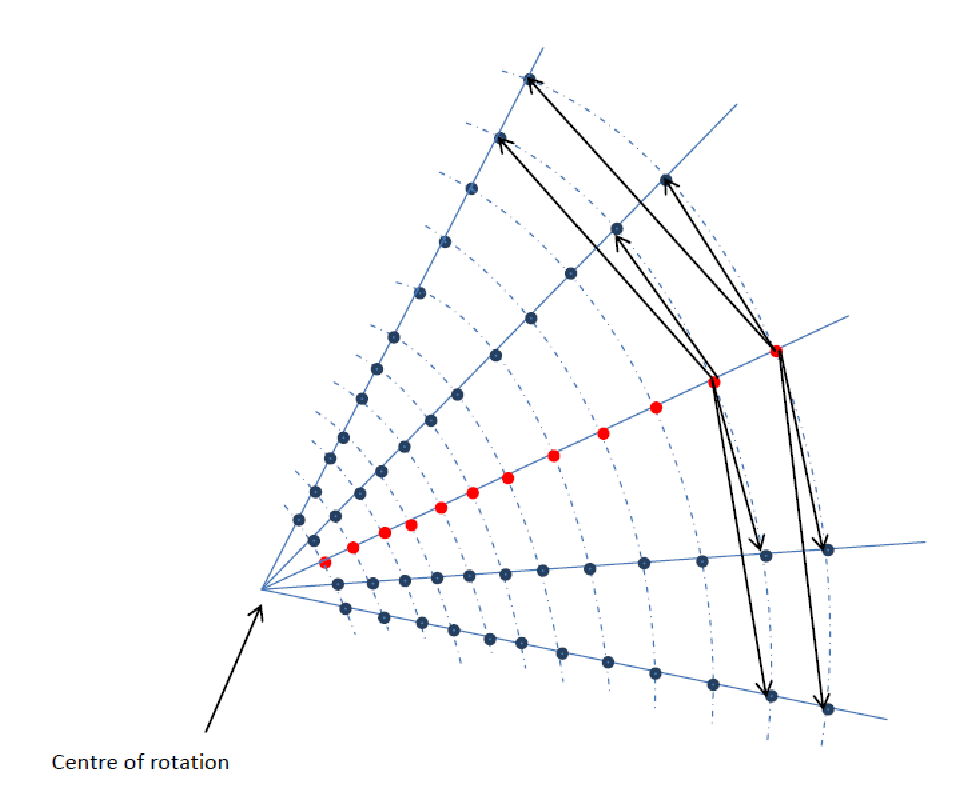
\includegraphics[width=1\columnwidth]{./Figures/uvcov.png}\caption{Schematic of $uv$-coverage for 
regularly spaced time-frequency samples.}\label{fig:uvcov}
\end{figure}


\subsection{Effect of averaging on the image}
\label{sec:effectbw}

\begin{figure*}
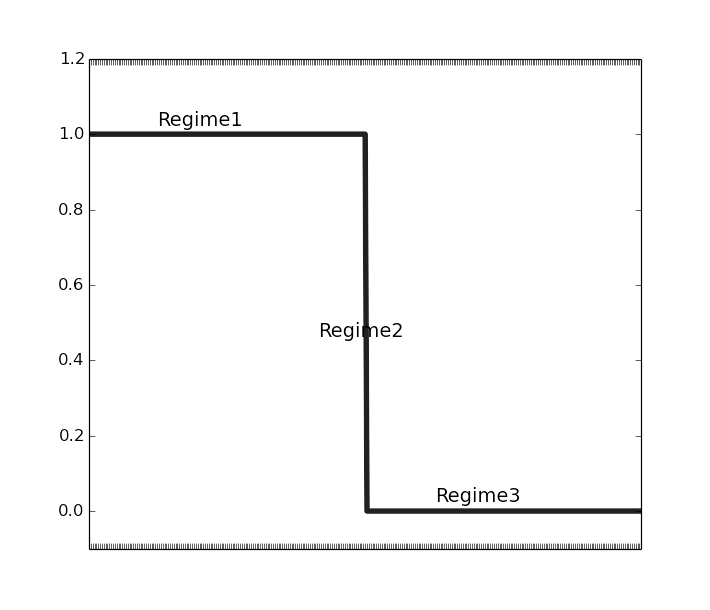
\includegraphics[width=.4\textwidth]{./Figures/idealIPRgrey.png}%
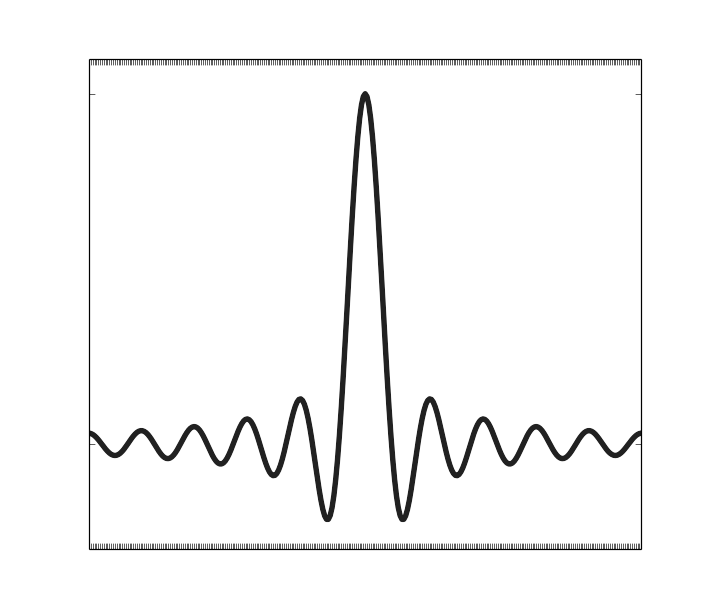
\includegraphics[width=.4\textwidth]{./Figures/idealsincgrey.png}\\
\caption{Left: boxcar response. In the $uv$-plane, this represents the windowing function corresponding to normal
averaging of visibilities. In the image plane, this represents the ideal image-plane tapering function. Right: 
Sinc response. In the image plane, this represents the tapering function corresponding to a boxcar WF in 
the $uv$-plane. In the $uv$-plane, this represents the ideal WF.}
\label{fig:idealWF}
\end{figure*}

In the limit of $\Delta t,\Delta \nu \rightarrow 0$, averaging becomes equivalent to sampling. 
An interferometer must, intrinsically, employ a finitely small averaging interval. The Fourier phase 
component $2\pi\phi(u,v,w)$ is a function of frequency and time, with increasing variation over the averaging interval 
for sources far from the phase centre. The average of a complex quantity with a varying phase then effectively ``washes out'' 
amplitude, the effect being especially severe for wide FoVs \citep[for an extensive discussion, see][]{bregman2012system}. This
effect is often referred to as \emph{time} and \emph{bandwidth smearing}.

The discussion above provides an alternative way to look at smearing. Combining eqs.~(\ref{eq:imaging}--\ref{eq:imaging:DI}) with 
(\ref{eq:avscon}), and using the Fourier convolution theorem, we can see that the dirty image is formed up as
\begin{equation}
\IID =  \sum_{pqkl} W_{pqkl}  \TT_{pqkl} \IIDI_{pqkl},
\end{equation}
where the baseline-dependent \emph{tapering function} $\TT_{pqkl}$ is the inverse FT of the BDWF:
\begin{equation}
\TT_{pqkl} = \FF^H\{ \Puv_{pqkl} \}.
\end{equation}
In other words, the dirty image made from averaged visibilities is a weighted average of the per-visibility ideal dirty images, 
each one multiplies by its own taper. The FT of a boxcar-like function is a sinc-like function, schematically illustrated in one
dimension by Fig.~\ref{fig:idealWF}. Time and bandwidth smearing represents the average effect 
of all these individual tapers. Shorter baselines correspond to smaller boxcars and wider tapers, longer baselines to larger 
boxcars and narrower tapers, and are thus more prone to smearing.

\begin{figure*}
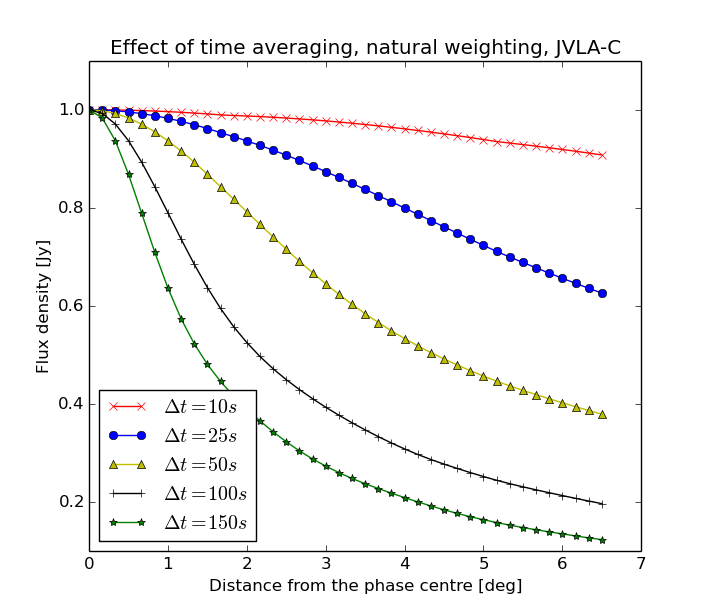
\includegraphics[width=\columnwidth]{./Figures/effect_time_averaging.png}%
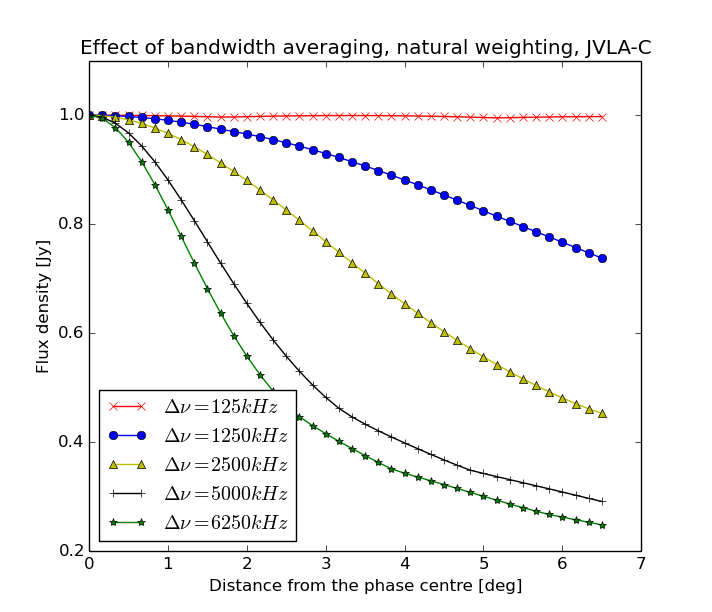
\includegraphics[width=\columnwidth]{./Figures/effect_bandwidth_averaging.png}
\caption{Effects of time and frequency averaging: the apparent intensity of a 1 Jy source, as seen by JVLA-C at 1.4 GHz, 
as a function of distance from phase centre. (Left) Frequency interval fixed at 125 kHz, time interval varies; 
(right) time interval fixed at 1s, frequency interval varies.}\label{fig:smear}
\end{figure*}

Figure \ref{fig:smear} (produced by simulating a series of high time-frequency resolution observation using MeqTrees, and 
applying averaging) shows the attenuation of a 1 Jy source as a function of distance
from phase centre, for a set of different time and frequency intervals. The simulations correspond to JVLA 
in the C configuration, with an observing frequency of 1.4 GHz. At this frequency, the first null of the PB is at 
$r\approx36'$, and the half-power point is at $\sim16'$, thus we can consider the ``conventional'' FoV (i.e. the half-power 
beam width, or HPBW) to be about $0.5^\circ$ across. Note that the sensitivity of the upgraded JVLA, as well as
improvements in calibration techniques \cite{Perley2013}, allow imaging to be done in the first PB sidelobe as well
(and in fact it may be necessary for deep pointings, if only to deconvolve and subtract sidelobe sources), so we could also
consider an ``extended'' FoV extending out to the second null of the PB at $r\approx1.25^\circ$. Whatever definition
of the FoV we adopt, Fig.~\ref{fig:smear} shows that to keep amplitude losses across
the FoV to within some acceptable threshold, say 1\%, the averaging interval cannot exceed some critical size,
say 10s and 1 MHz. Conversely, if we were to adopt an aggressive averaging strategy for the purposes of data 
compression, say 50s and 5 MHz, the curves indicate that we would suffer substantial amplitude loss towards the 
edge of the FoV. 

Finally, note that the curves corresponding to acceptably low values of smearing across the FoV (i.e. up to 25s and 
up to 1.25 MHz) have a very gentle slope, with very little suppression of sources \emph{outside} the FoV. 

\subsection{The case for alternative BDWFs}

The tapering response induced by normal averaging (Fig.~\ref{fig:smear}) is far from ideal: it either suppresses too much within 
the FoV, or too little outside the FoV, or both. The optimal tapering response would be boxcar-like, as in 
Fig.~\ref{fig:idealWF}(left). The BDWF that would produce such a response is sinc-like, as in Fig.~\ref{fig:idealWF}(right). 
The problem with a sinc is that it has infinite support; applying it over finite-sized bins necessarily means a \emph{truncated} 
BDWF that results in a suboptimal taper. The problem of optimal filtering has been well studied in signal processing (usually
assuming a true convolution rather than the pseudo-convolution we deal with here), and we shall apply these lessons below.

The derivations above make it clear that by using a different BDWF in place of the conventional boxcar-like $\Puv$ 
could in principle yield more optimal tapering response. The obvious catch is a loss in 
sensitivity. Each visibility sample is subject to an independent Gaussian noise term in the real and imaginary part; the noise of
the average of a set of samples is minimized when the average is naturally weighted (or unweighted, if the noise is 
constant across visibilities). Thus, any deviation from a boxcar WF must necessarily increase the noise in the 
visibilities. Below we will study this effect both theoretically and via simulations, to establish whether this 
trade-off is sensible, and under which conditions.

\section{Overview of windowing functions}
\label{subsec:Windowing functions}

In signal processing (SP), a WF is a mathematical function with limited support (i.e. zero outside some interval). Conventionally,
a time series is convolved with a WF to produce some desired response in the frequency domain. Applying this to our problem
can lead to quite some confusion in terminology. Table~\ref{tab:terms} provides a mapping between the terms commonly used in SP, 
and their conceptual equivalent in BDWFs.

\begin{table}
\begin{tabular}{l|l}
\hline
 \bf Signal processing & \bf BDWFs\\
\hline\hline
Frequency (freq) domain & Image plane \\
Time domain & Fourier plane or $uv$ plane \\
Spectral response\\
~~or freq response & Image plane response (IPR)\\
Time response & Fourier plane response\\
Cut-off time interval  \\
~~or time pass band & $uv$ averaging bin\\
Cut-off freq interval \\
~~or freq pass band, or main lobe & FoV\\
Time stop band & Outside of the $uv$-bin\\
Freq stop band & Outside of the FoV\\
Octave & Doubling in size\\
Normalized freq & Distance from phase centre \\
Band-limited \\
~~(applied to visibilities) & restricted FoV \\
\end{tabular}
\caption{Mapping of terminology between signal processing and BDWFs.}
\label{tab:terms}
\end{table}


WF -- or rather their corresponding image-plane response (IPR) -- can be characterized in terms of various metrics. Some common 
ones are the peak sidelobe level (PSL), the main lobe width (MLW) and the sidelobes roll-off (SLR) rate. In terms of the ``ideal'' 
IPR (Fig.~\ref{fig:idealWF}, left), these correspond to the following desirable traits:

\begin{itemize}
\item Maximally conserve the signal within the FoV (``regime 1'' in the figure), and make the transition in ``regime 2'' as sharp as possible. Both of these correspond to larger MLW.
\item Attenuate sources outside the FoV (``regime 3''): this corresponds to a lower PSL and higher SLR.
\end{itemize}

Below we provide an overview some common (one-dimensional) WFs employed in signal processing.

\newcommand{\FilterFigure}[4]{
\begin{figure}
\includegraphics[width=.5\columnwidth]{#1}%
\includegraphics[width=.5\columnwidth]{#2}
\caption{#3}\label{#4}
\end{figure}
}

\subsection{Boxcar window}

\FilterFigure{Figures/boxcargrey.png}{Figures/freq_resp_boxgrey.png}{Boxcar windowing 
function and its tapering response.}{fig:wf:box}

The boxcar window for a cut-off time interval of $[-t_a,t_a]$ is defined as:
\begin{equation}
\Pi(t)=\left\{
\begin{array}{rl}
1 & \mbox{$-t_a \leq t \leq t_a$} \\
0 & \mbox{otherwise}
\end{array}\right.
\end{equation}
Fig. \ref{fig:wf:box} shows a plot of $\Pi(t)$ and its response. The thick grey and thin curves 
correspond to cut-off time intervals of $[-t_a, t_a]$ and 
$[-t_a/2,t_a/2]$ respectively. Note that when the cut-off time interval is larger, the MLW is 
narrower, and the sidelobes are lower.

The other WFs given below are all multiplied with a boxcar to ensure a cut-off interval of $[-t_a,t_a]$.

\subsection{Gaussian window}

\FilterFigure{./Figures/gaussiangrey.png}{./Figures/freq_resp_gaussiangrey.png}{Gaussian 
windowing function and its tapering response.}{fig:wf:gauss}

A Gaussian WF centred at zero with a standard deviation of $\sigma_1$ is given by: 
\begin{equation}
\mathrm{G}(t)= \Pi(t) e^{-bt^{2}}, \label{eq:gauss}
\end{equation}
where $b=(2\sigma_1^2)^{-1}$. The FT of the Gaussian term is given by 
$\mathcal{F}\big\{\mathrm{G}\big\}=\sqrt{\frac{b}{\pi}}e^{-cl^2}$, where $c=\pi^2/b$, i.e.
is also a Gaussian with standard deviation of $\sigma_2= (2\pi\sigma_1)^{-1}$.

Fig. \ref{fig:wf:gauss} shows a plot of $\mathrm{G}(t)$ and its response. 
The WF is truncated at $[-t_a,t_a]$, with $b = 3$ for the thin curve and $b=5$ for the thick grey curve. 
Its response is characterized by extremely low sidelobes, but a narrow main lobe.

\subsection{Butterworth window}

\FilterFigure{./Figures/butterworthgrey.png}{./Figures/freq_resp_butterworthgrey.png}{Butterworth 
windowing function and its tapering response.}{fig:wf:bw}

A Butterworth WF is flat in the time pass band, and rolls off towards zero in the time stop band and it is 
characterized by two independent parameters, the cut-off time time $[-t_a,t_a]$ and the order $p$. 
The two parameters control the 
FoV and sidelobes attenuation. The Butterworth WF is given by:
\begin{equation}
\mathrm{BW}(t)= \Pi(t) \Big(1 + (t/t_a)^{2p}\Big)^{-1}.
\end{equation}

Figure \ref{fig:wf:bw} shows Butterworth WFs for the same cut-off interval $[-t_a,t_a]$, with orders of $p=1,3$. Note that increasing 
the order $p$ conserves the MLW, and dramatically lowers distant sidelobes, at the cost of pushing up the near-in sidelobes

\subsection{Prolate spheroidal window}

\FilterFigure{./Figures/prolategrey.png}{./Figures/freq_resp_prolategrey.png}{Prolate 
spheroidal wave (of oder zeros) windowing function and its tapering response.}{fig:wf:prolate}

This WF is given by a prolate spheroidal wave function of sequence zero ($n=0$) characterized
by two independent parameters, the cut-off time $[-t_a,t_a]$ and the order $\alpha$ 
\citep{delsarte1985discrete, walter2006prolate}. 
The two parameters control the  FoV and sidelobes attenuation.
The prolate spheroidal wave function $\mathrm{PS}_0$ is the eigenfunction and solution of the integral:
\begin{equation}
\int\limits_{-t_a}^{t_a} \mathrm{PS}_{0}(\xi) \frac{sin(\frac{\alpha}{\pi}(t-\xi))}{\frac{\alpha}{\pi}(t-\xi)}d\xi=\lambda_{n=0,\alpha,t_a}\mathrm{PS}_{0}(t), 
\end{equation}
where $\lambda_{n=0,\alpha,t_a}$ is the coresponding eigenvalue. Fig. \ref{fig:wf:prolate} shows prolate 
spheroidal WFs for the same cut-off interval $[-t_a,t_a]$, with orders of $\alpha=2\pi^3, 5\pi^3$. 
Note that increasing the order $\alpha$ increases the MLW, and dramatically lowers sidelobes.

\subsection{Sinc window}

\FilterFigure{./Figures/sincgrey.png}{./Figures/freq_resp_sincgrey.png}{Sinc 
windowing function and its tapering response.}{fig:wf:sinc}

The sinc WF is defined as 
\begin{equation}
\mathrm{Sinc}(t)= \Pi(t) \frac{\sin(\pi b t)}{\pi b t} .
\end{equation}
Fig. \ref{fig:wf:sinc} shows $\mathrm{Sinc}(t)$ for a fixed value of $b$, and cut-off intervals given 
by $[-t_a,t_a]$ and $[-t_a/2,t_a/2]$. Note that the response to a sinc WF is almost perfectly flat in the main lobe (more so for larger intervals). The sidelobe response is relatively poor, but better for larger intervals.

\subsection{Bessel $J_0$ window}
\label{Bessel}
\FilterFigure{./Figures/besselgrey.png}{./Figures/freq_resp_besselgrey.png}{$J_0$ 
windowing function and its tapering response.}{fig:wf:bessel}

This WF is given by a Bessel function of the first kind of order zero \citep{watson1995treatise}. Using a power series expansion, we have:
\begin{equation}
J_0(t) = \Pi(t) \sum_{k=0}^{\infty}\frac{(-1)^k (t/2)^{2k}}{(k!)^2}.
\end{equation}
Fig. \ref{fig:wf:bessel} shows $J_0(t)$ and its response, with $J_0(t)$ truncated at time intervals $[-t_a,t_a]$ and 
$[-t_a/2,t_a/2]$. The performance of $J_0$ is somewhat worse than the sinc within the main lobe, and somewhat better in
the sidelobes.

\begin{figure*}
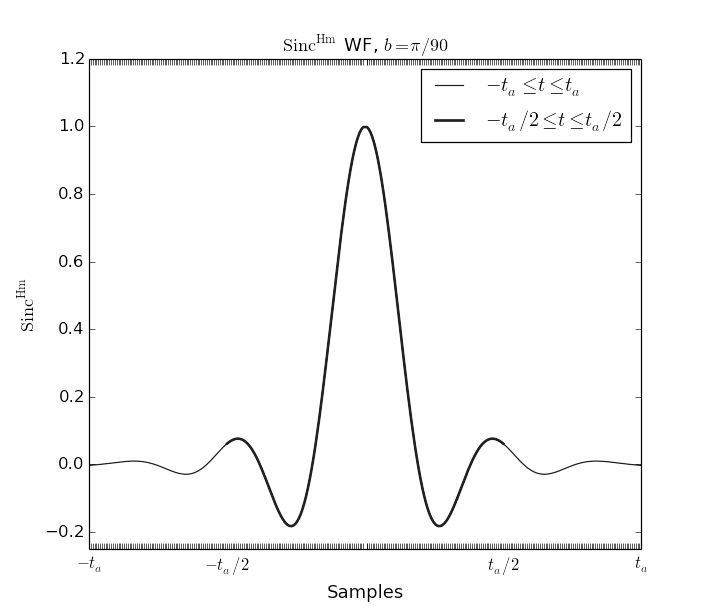
\includegraphics[width=.25\textwidth]{./Figures/sinc-hamminggrey.png}%
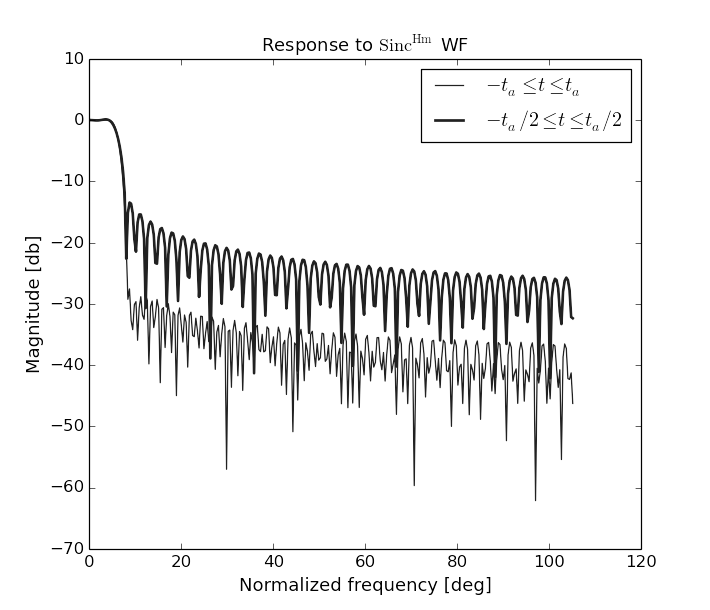
\includegraphics[width=.25\textwidth]{./Figures/freq_resp_sinc-hamminggrey.png}%
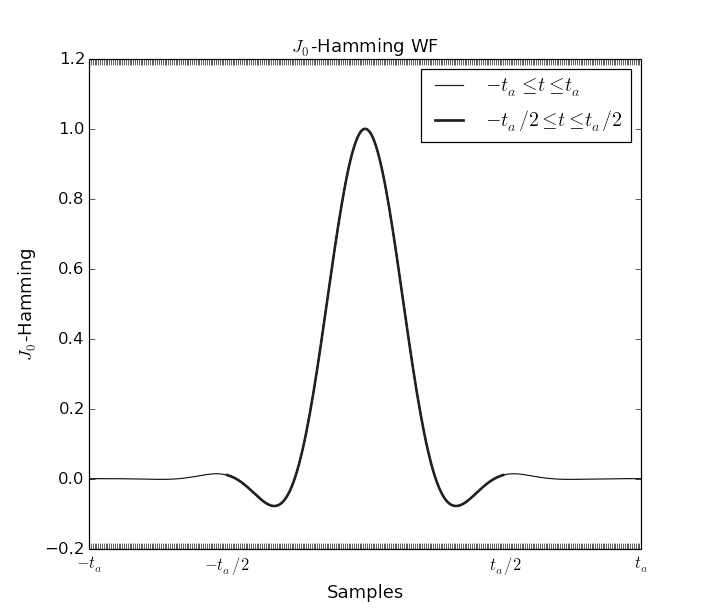
\includegraphics[width=.25\textwidth]{./Figures/bessel-hamminggrey.png}%
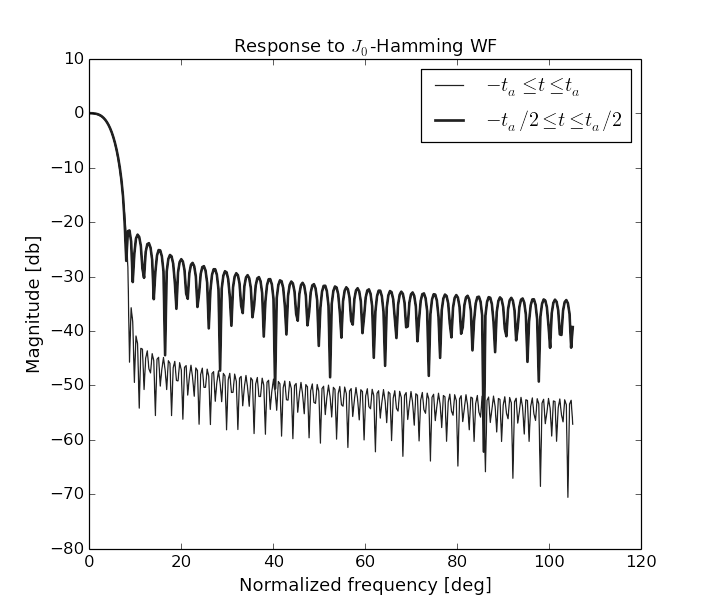
\includegraphics[width=.25\textwidth]{./Figures/freq_resp_bessel-hamminggrey.png}%
\caption{Sinc-Hamming and it tapering response (the two left plots) as well as the Bessel-Hamming (the two right plots).}\label{fig:wf:JhSh}
\end{figure*}

\subsection{Sinc-Hamming and $J_0$-Hamming windows}

% \OMS{Marcellin, this is contradictory. If you're passing the signal through two filters as you say, that means 
% two convolutions. But here you write the WF as a product of $J_0$ with another function. That's convolution with a 
% product, not two convolutions. So which one is correct? Also, please provide citations for the Hanning, Hamming and 
% Blackman filters. Also, in the figures the WFs look absolutely identical. Is this an error, or are they really so similar?
% If the latter, then we really shouldn't waste space... \\Marcellin: corrected. it is one convolution not two.
% Thank you for drawing my intention. Yes they are very similar, I prefer to present two cases,
% the Bessel-Hamming and sinc-hamming. See text}
Depending on the science goals we want to achieve, the Hamming, Hanning or Blackman filter is sometime multiplied by 
a $J_0(t)$ or $\mathrm{Sinc}(t)$ to increase the pass band (regime 1 or FoV) and 
increase the stop band (regime 3 or outside the FoV) attenuation.
% A $J_0(t)$ WF can be used to filter out the input signal as previously mentioned. . The intermediate signal 
% can then be passed through a Hamming, Hanning or Blackman filter to further increase the pass band (regime 1 or FoV) and 
% increase the stop band (regime 3 or outside the FoV) attenuation. 
The process can be resume as follow:
\begin{equation}
Y^\mathrm{X} = Y(t) X(t) 
\end{equation}
where $X(t)$ is either the Hamming (Hm), Hanning (Hn) or Blackman (B) WFs well known in SP litterature
\citep{nuttall1982spectral,podder2014comparative} and $Y$ is a $J_0(t)$ or $\mathrm{Sinc}(t)$ WF.
% \OMS{citation please. Marcellin: correction done}.
Fig. \ref{fig:wf:JhSh} shows the $J_0^\mathrm{Hm}, \mathrm{Sinc}^\mathrm{Hm}$ WFs and their responses. Compared to the $J_0(t)$ and 
$\mathrm{Sinc}(t)$, they show lower PSL and higher SLR.

\subsection{Relative performance}
% \subsection{Convolution theorem and WFs comparison}
% We begin with a continuous signal $V_{t}$ (supposed the data is only time dependent) and sample it in order to obtain the set of 
% measurement (see section \ref{sec:AvgCon}). When the signal is limited in the time interval $[-t_a,t_a]$ and convolved with a window 
% $W_{t}$, it 
% follows from the convolution theorem that the process was equivalent to "\textit{tapering the  Fourier transform of the signal}" by 
% effectively looking at the true Fourier transform of the signal through the convolution window. This is presented mathematically as:
% \begin{equation}
% \mathcal{F}\Big\{V_{t}\circ W_{t}\Big\} = \mathcal{F}\Big\{V_{t}\Big\}\cdot \mathcal{F}\Big\{W_{t}\Big\}
% \end{equation}
% One can replaced the convolution window, $W_{t}$ by its Fourier transform. A summary of the MLW, the PSL and 
% the SLR of the windows study is showed in table below.
\begin{table}
\begin{tabular}{|l||l|l|l|l|}
\hline
 \bf WFs& &\bf{Windows} & \bf response\\
 &&{ MLW} & { PSL}  & { SLR}   \\
  &&\hspace{-0.8cm}(deg and at -3db) & (db) & (db/oct)  \\
\hline\hline
{$\Pi(t)$}  & $t\in|t_a|$& $\sim 1.406$ &$-6.663$ &$-12.089$\\
	    & $t\in|t_a/2|$&$\sim 2.812$ &$-6.671$ &$-11.065$\\
\hline
{$\mathrm{Sinc}(t)$} & $t\in|t_a|$ &$\sim 12.304$& $-10.889$&  $-12.661$ \\
	 & $t\in|t_a/2|$ &$\sim 12.304$& $-13.241$&  $-11.447$ \\
\hline
{$J_0(t)$}& $t\in|t_a|$ &$\sim 9.140$ &$ -14.553$ & $ -12.011$\\
	  & $t\in|t_a/2|$ &$\sim 9.140$ &$ -13.614$ & $ -11.794$\\
\hline
{$\mathrm{G}(t)$} & b=3 &$\sim 2.109$& $-21.535$& $-9.589$\\ 
	 & b=5 &$\sim 2.812$& $-30.211$& $-9.091$\\ 
\hline
{$\mathrm{BW}(t)$} & p=1 &$\sim 2.109$ &$-13.718$ & $-12.581$\\
	  & p=3 &$\sim 4.218$ &$-10.145$ & $-27.330$\\
\hline
{$\mathrm{PS}_0(t)$} & $\alpha=2\pi^3$ &$\sim 3.515$& $-45.302$& $-7.424$\\ 
	 & $\alpha=5\pi^3$ &$\sim 4.218$& $-73.597$& $-6.375$\\ 
\hline
{$J_0^\mathrm{Hm}(t)$} & $t\in|t_a|$ &$\sim 9.140$&$-35.724$ & $-11.948$\\ 
 & $t\in|t_a/2|$ &$\sim 9.140$&$-22.670$&$-19.527$\\ 
\hline
{$Sinc^\mathrm{Hm}(t)$}  & $t\in|t_a|$ &$\sim 12.656 $&$-27.581$ &$-13.817$ \\ 
 &$t\in|t_a/2|$ &$\sim12.656$&$-13.469$&$-14.324$
\end{tabular}
\caption{\label{tab:WF:performance}Comparative performance of 
different windowing functions.}
% \OMS{Marcellin, it is not clear what exact variation of the
% WF these numbers correspond to. Maybe add a few rows for different variations (i.e. different values
% of $p$, $b$)? In fact, it's not even clear if the comparison is systematic. For example, the FoV realized 
% by different WFs is different.}
% \emph{ Marcellin anwser, thank you I noticed that when I was doing the new plots, I'll do it explicitly and 
% I want to change the scaling of the windows so that we can easily see what you are asking.}
\end{table}
Table~\ref{tab:WF:performance} summarizes the performance of the different WFs. From this it is clear that
the sinc and the Bessel ($J_0$) WFs provide the more optimal tapering response. It is these WFs that
will serve as the basis of BDWFs developed in the rest of this work. 

To construct two-dimensional BDWFs from one-dimensional WFs, we will use the following definitions:
\begin{eqnarray}
S(u,v) &=& S(u)S(v), \nonumber\\
J_0(u,v) &=& J_0(r), ~~~r=\sqrt{u^2+v^2}.\nonumber
\end{eqnarray}
% \OMS{Marcellin, why not $\mathrm{sinc}(r)$ as well? The referee is bound to ask? Also, why did you never consider a 
% prolate spheroidal WF? I remember bringing it up a few times. Marcellin: $\mathrm{sinc}(r)$ dosn't works well in signal recovery. I studied the prolate spheroidal wave functions(PSWF)
% and the oder 1 of PSWF was just slightly like the sinc but with low sidelobes. I can try and test this but for sure 
% the computational time is extremely huge. I was thinking to talk about 
% the Hamming*[sinc or bessel], Hinning*[sinc or bessel], blackman*[sinc or bessel] there are also performing well.}

\section{Application of WFs to visibilities}

While visibilities are (usually) regularly sampled in $t\nu$-space, in $uv^\mathrm{m}$-space this is not so. In frequency, 
the sampling positions go as $\sim\nu^{-1}$, while in time, baselines with a longer East-West component sweep out longer tracks between successive 
integrations (Fig.~\ref{fig:uvcov}). Applying a WF with a constant integration window in $t\nu$ space corresponds to 
different-sized windows in $uv$-space. In the case of normal averaging, this results in the boxcar-like window $\Puv$ of 
eq.~(\ref{eq:avscon}) having a baseline-dependent scale. The scale of the tapering response being inversely proportional to 
the scale of the WF, this results in more smearing (i.e. a narrower FoV) on longer baselines.

By defining our alternative WFs in $uv$-space (in units of wavelength), we can attempt to ``even out'' the smearing 
response across baselines. For a given BDWF $X(u,v)$, we have the following recipe 
for computing resampled visibilities (compare to eq.~\ref{eq:discrete:uv}):
\begin{equation}
\label{eq:avg:wf}
V^\mathrm{(m)}_{pqkl} = \frac{\displaystyle\sum\limits_{{i,j}\in \Bij_{kl}} \Vs_{pqij} X(\bmath{u}_{pqij}-\bmath{u}_{pqkl})}
{\displaystyle\sum\limits_{{i,j}\in \Bij_{kl}} X(\bmath{u}_{pqij}-\bmath{u}_{pqkl})},
\end{equation}
where $\bmath{u}_{pqkl}$ is the midpoint of the resampling bin $\Bij_{kl}$ in $uv$-space. The main lobe of the WF then 
has the same scale across the entire $uv$-plane, while the resampling bins have different $uv$-sizes. Conversely, in 
$t\nu$-space the bins
are regular, while the main lobe of the effective WF scales inversely with the baseline fringe rate. Furthermore, 
the WF is truncated at the edge of each bin; on the shortest baselines this truncation is extreme to the 
point of approaching the boxcar-like $\Puv$ (Fig.~\ref{fig:WF:perbaseline}).

\begin{figure*}%
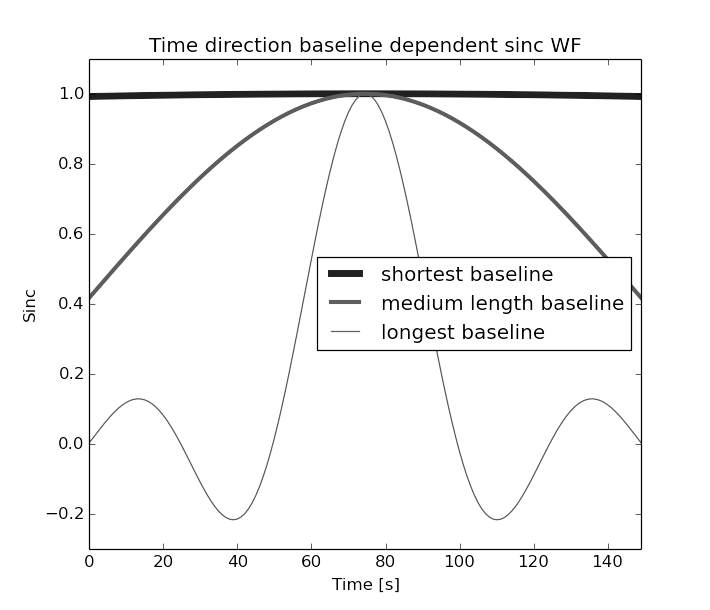
\includegraphics[width=.4\textwidth]{./Figures/sinc-baseline_longMidShortshortgrey.png}%
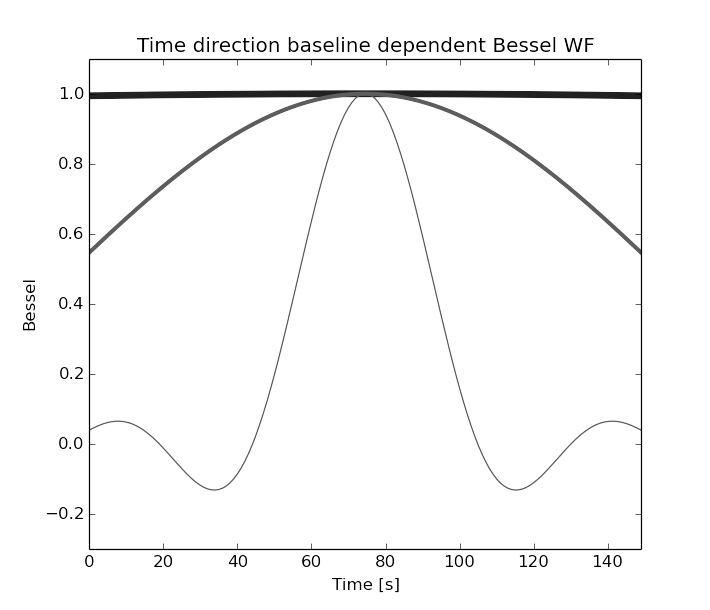
\includegraphics[width=.4\textwidth]{./Figures/bessel-baseline_longMidShortshortgrey.png}
%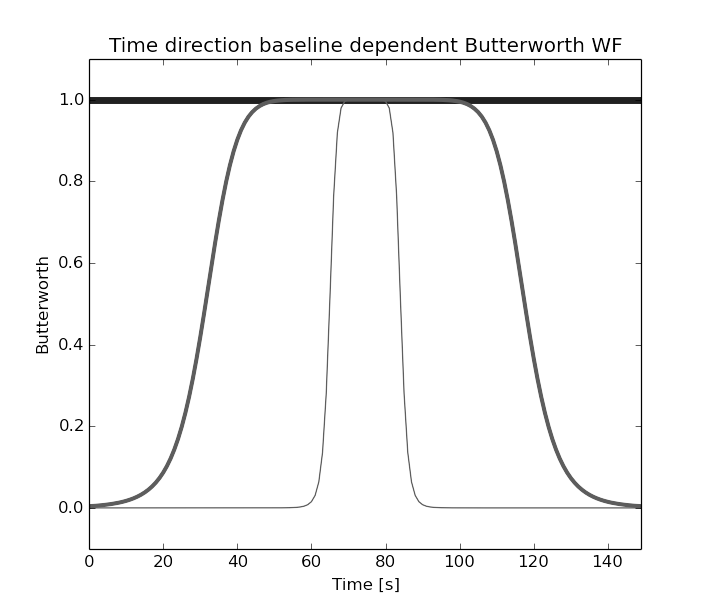
\includegraphics[width=.33\textwidth]{./Figures/butterworth-baseline_longMidShortshortgrey.png}
\caption{Cross-sections through two different BDWFs (left: sinc, right: Bessel) defined in $uv$-space, 
plotted along the time axis. This shows that the effective WF is a scaling and truncation of the underlying WF, with
the shortest baselines reducing to a boxcar-like WF.
% \OMS{Marcellin please make the PDF figures greyscale, and the same size.
% Also please leave legend on only one of them, it's redundant.Marcellin: correction done}
}
\label{fig:WF:perbaseline}
\end{figure*}

The downside of this simple approach is twofold. Firstly, while all of the WFs above nominally exhibit far lower 
sidelobes than the boxcar
(i.e. more suppression for out-of-FoV sources), they no longer perform that well under truncation, with extremely truncated WFs 
at the shorter baselines becoming boxcar-like. Secondly, taking a weighted sum in eq.~\ref{eq:avg:wf} increases 
the noise in comparison to normal averaging.

\subsection{Bin sizes}

\OMS{Note to self: Talk about time-frequency bins sizes here. Also about tunable FoVs.}


\subsection{Overlapping BDWFs}
\label{baseline2}
\newcommand{\WF}[3]{{#1}-$#2${}$\times${}$#3$}
\begin{figure} 
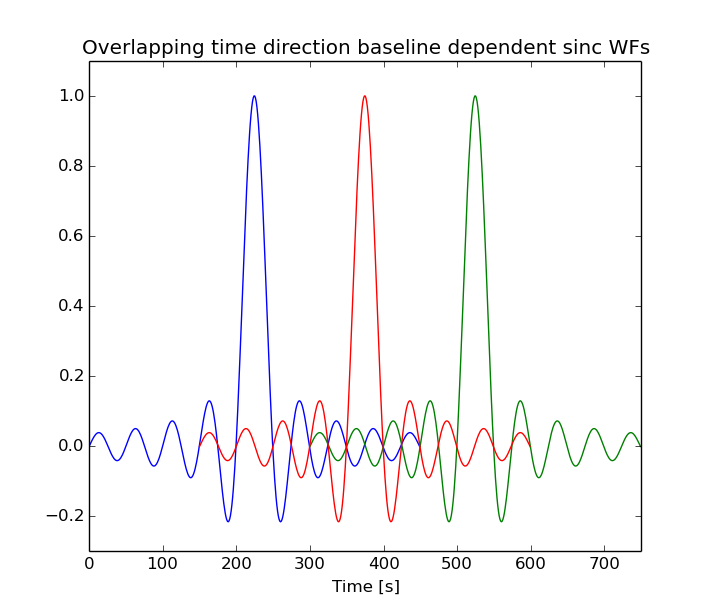
\includegraphics[width=\columnwidth]{./Figures/corrSigVLAMxBl_overlapGdelta.png}\caption{Overlapping 
BDWFs representing adjacent resampling bins. This corresponds to overlap factor $\alpha=3$ in time.}\label{fig:overlap}
\end{figure}

A more sophisticated approach involves overlapping BDWFs. Normal averaging implicitly assumes that the resampling bins $B_{kl}$ 
in eq.~(\ref{eq:avg:wf}) don't overlap for adjacent $kl$, since they represent adjacent averaging intervals. 
There is, however, no reason (apart from computational load) why we cannot take the sum in eq.~(\ref{eq:avg:wf}) 
over larger bins. Let us define the \emph{windowing bin} for \emph{overlap factors} of $\alpha,\beta$ as
\begin{equation}
\Bab_{kl} = \big \{ ij:~t_i\nu_j \in \Babtf_{kl} \big \},
\end{equation}
i.e. as the set of sample indices corresponding to a bin of size $\alpha\Delta t\times\beta\Delta \nu$ in $t\nu$-space.
Let us then compute the sums in eq.~(\ref{eq:avg:wf}) over the windowing bin. This becomes distinct from the
resampling bin: while the latter represents the spacing of the resampled visibilities, the former represents the size 
of the window over which the convolution is computed. Only for $\alpha=\beta=1$ do the two bins become the same.

BDWFs in the overlapping regime are schematically illustrated in Fig.~\ref{fig:overlap}. For normal averaging 
overlapping offers no benefit, since it only broadens $\Puv$ and therefore increases smearing. But for a well-behaved 
BDWF, enlarging the windowing bin (while maintaining the same WF scale) means less truncation -- thus lower 
sidelobes -- and decreased noise, as more sampled visibilities are taken into account.

To distinguish overlapping BDWFs from non-overlapping ones, in the rest of the paper we will designate the 
WFs employed as \WF{\em WF}{\alpha}{\beta}. For example, \WF{sinc}{3}{2}, \WF{$J_0$}{1}{1} (i.e. no overlap), etc.
If resampling is only done in one direction (only time or only frequency), we'll indicate this as e.g. \WF{$J_0$}{3}{-}.

\subsection{Noise penalty estimates: analytic}
\label{sec:imaging}
% \OMS{Marcellin, I can't follow the old derivations, and neither will the referee I fear. 
% The idea is solid, but your notation is a bit of a mess. Need to straighten it out
% and express in terms of Sect.~2.2, i.e. lo-res (averaged) and hi-res (sampled) visibilities. 
% Suggest also working it out for the unpolarized case instead, you can then drop the 
% extra ``4'' in the dimensions and simplify the matrices. Also, you need to explain, what is $N_t$ and $n_t$? 
% Maybe it makes sense to leave the complicated derivations for your thesis, and go with something simple here. 
% For example:}

Let us now work out analytically the \emph{noise penalty} associated with replacing an unweighted average by 
a weighted sum. For simplicity, let's assume that the noise term
has constant r.m.s. $\sigma_\mathrm{s}$ across all baselines and samples. If the resampling bin 
consists of $n_\mathrm{avg} = n_t\times n_\nu$ samples, and since the noise is not correlated between samples, 
the noise on the averaged visibilities in eq.~(\ref{eq:discrete:tf0}) will be given by
\begin{equation}
\sigma_\mathrm{m}^2 = \frac{1}{n_\mathrm{avg}^2} \sum_{i=1}^{n_\mathrm{avg}} \sigma_\mathrm{s}^2  = \frac{\sigma_\mathrm{s}^2}{n_\mathrm{avg}}
\end{equation}
Note that the noise is uncorrelated across averaged visibilities. We can therefore use the
the imaging equation (\ref{eq:imaging3}) to derive the following expression for the variance of the noise 
term in each pixel of the dirty image:
\begin{equation}
\label{eq:noise:image}
\sigma_\mathrm{pix}^2 = \frac{ (\sum_{pqkl} W_{pqkl}^2 \sigma_\mathrm{m}^2) }{ (\sum_{pqkl} W_{pqkl})^2 },
\end{equation}
which for natural image weighting ($W\sim\sigma^{-1}_\mathrm{m}$, i.e. $W\equiv1$ in this case) is simply
\begin{equation}
\sigma_\mathrm{pix}^2 = \frac{1}{N}\frac{\sigma_\mathrm{s}^2}{n_\mathrm{avg}},
\end{equation}
where $N$ is the total number of visibilities used for the synthesis.

To simplify further notation, let's replace $pqkl$ by a single index $\mu$, enumerating all the lo-res visibilities $\Vm_\mu$, with 
$\mu=1\dots N$. If we now employ eq.~(\ref{eq:avg:wf}) to compute the lo-res visibilities using some BDWF $X(u,v)$, the noise 
term becomes different per each visibility $\mu$:
\begin{equation}
\label{eq:noise:bdwf}
\sigma_{X\mu}^2 = \frac{\sum X^2(\bmath{u}_{pqij}-\bmath{u}_{pqkl})}
{\big [ \sum X(\bmath{u}_{pqij}-\bmath{u}_{pqkl}) \big ]^2 } \, \sigma_\mathrm{s}^2
\end{equation}
where both sums are taken over the windowing bin, ${i,j}\in \Bij_{kl}$. Let us define 
the \emph{visibility noise penalty} associated with BDWF $X$ 
and visibility $\mu$ as the relative increase in noise over the unweighted average, i.e.
\begin{equation}
\Xi_{X\mu} = \frac{\sigma_{X\mu}}{\sigma_\mathrm{m}} = 
\frac{ \sqrt{ n_\mathrm{avg} \sum X^2(\bmath{u}_{pqij}-\bmath{u}_{pqkl}) }}
{\sum X(\bmath{u}_{pqij}-\bmath{u}_{pqkl}) }. 
\end{equation}
Note that in the case of overlapping BDWFs, the windowing bin in eq.~\ref{eq:noise:bdwf} is larger than the 
resampling bin, and contains $n_X$ samples, with $n_X=\alpha\beta n_\mathrm{avg}$, where $\alpha$ and $\beta$ are the 
overlap factors. For $\alpha=\beta=1,$ it is easy to see that $\Xi_{X\mu}\geq1$, and only reaches 1 when $X\equiv1$. 
In other words, non-overlapping BDWFs always result in a visibility noise penalty above 1, while overlapping BDWFs 
can actually \emph{reduce} noise in the resampled visibilities. 

While paradoxical at first glance, this reduction in noise does {\bf not} result in a net gain in image 
sensitivity. The reason for this is that with overlap in effect, the noise terms become correlated across 
resampled visibilities $kl$ (within the same baseline $pq$), with each hi-res visibility sample contributing to 
multiple resampled visibilities, and the image noise term no longer follows eq.~(\ref{eq:noise:image}).

If the resampled visibilities correspond to a single-channel snapshot, or if the BDWFs are non-overlapping,
then the noise across visibilities remains uncorrelated, and we can compute the \emph{image noise penalty} 
associated with imaging weights $W$ and BDWF $X$ as
\begin{equation}
\Xi^W_X = 
\frac{\sigma_{\mathrm{pix},X}^2}{\sigma_{\mathrm{pix}}} = \frac{n}{\sigma_\mathrm{s}}
\frac{ (\sum_{\mu} W_{\mu}^2 \sigma_\mu^2) }{  (\sum_{\mu} W_{\mu})^2 } =
\frac{ (\sum_{\mu} W_{\mu}^2 \Xi_{X\mu}^2) }{ (\sum_{\mu} W_{\mu})^2 } 
\end{equation}

In the case of natural weighting ($W_\mu=\sigma_\mu^{-1}$) this reduces to:
\begin{equation}
\label{eq:noisepenalty:natural}
\Xi_X^{\mathrm{nat}} = \frac{N}{ \sum_{\mu} \Xi_{X\mu}^{-1} }.
\end{equation}

% \OMS{the matrix-based formalism that I commented out for now can actually deal with the overlap (correlated noise) 
% case, so it will be good to clean it up and include it in your thesis. If you clean it up sufficiently quickly for
% publication, we can also include it here.}

\subsection{Noise penalty estimates: empirical}

\label{subsec:noise}
In this section we employ simulations to empirically verify noise estimates computed using the derivation 
above. We generate a ``high-res''
JVLA-C measurement set corresponding to a 400s synthesis with 1s integration, with 30 MHz of bandwidth
centred on 1.4 GHz, divided into 360 channels of 83.4 kHz each. The MS is filled with simulated thermal noise 
with $\sigma_\mathrm{s}=1$ Jy. We then generate a ``low-resolution'' MS using 100s integration, with 
a single frequency channel of 10 MHz. This MS receives the resampled visibilities. 
The size of the resampling bin is thus 100s by 10MHz, or $100\times120$ in terms of the number of hi-res samples.

We then resample the hi-res visibilities using a number of BDWFs, and store the results in the lo-res MS:

\begin{itemize}
\item Standard averaging to 100s and 10MHz (using the middle 120 channels). This gives us the baseline noise
estimate.
\item Sinc and Bessel windows using the same bin, without an overlap, tuned to a FoV of $2^\circ$.
\item The same windows with overlap factors of $4\times3$.
\end{itemize}

We then image the lo-res MS and take the r.m.s. pixel noise across the image as an estimator of $\sigma_\mathrm{pix}$,
divide it by the baseline estimate produced with normal averaging, and compare the resulting noise penalty with that
predicted by eq.~\ref{eq:noisepenalty:natural}. Note that this estimator is not perfect, since image noise is correlated
across pixels. Nonetheless, we obtain results that are broadly consistent with analytical predictions 
(Table~\ref{tab:noise-comparison}).

Figure~\ref{fig:per-baseline-noise} shows the predicted visibility noise penalty for the same BDWFs, as a function of 
East-West baseline component, which determines the baseline rotation speed. Note that the noise penalty rises sharply towards 
longer E-W baselines. Note also that the penalty is well below 1 on shorter baselines, when overlapping is in effect.

\begin{table}
\begin{tabular}{lll}
\hline
{\bf BDWF} & {\bf $\Xi$ analytic } & {\bf $\Xi$ sim}\\
\hline\hline
\WF{sinc}{1}{1} &$1.247$ &$1.22$\\
%\WF{Sinc}{3}{2} &$1.02$ &$1.18$\\
\WF{sinc}{4}{3} &$1.242$ &$1.20$\\
\hline
\WF{besse}{1}{1} & $1.178$& $1.16$\\
%\WF{$J_0$}{3}{2} & $0.91$& $1.08$\\
\WF{bessel}{4}{3} & $1.109$& $1.12$\\
\hline
\end{tabular}
\caption{A comparison of image noise penalties associated with different BDWFs, computed analytically
vs. simulations. 
%\OMS{I find the <1 numbers for $J_0$ strange. Is this for a snapshot, or for the full 7m30s?}
}
\label{tab:noise-comparison}
\end{table}

\begin{figure*}
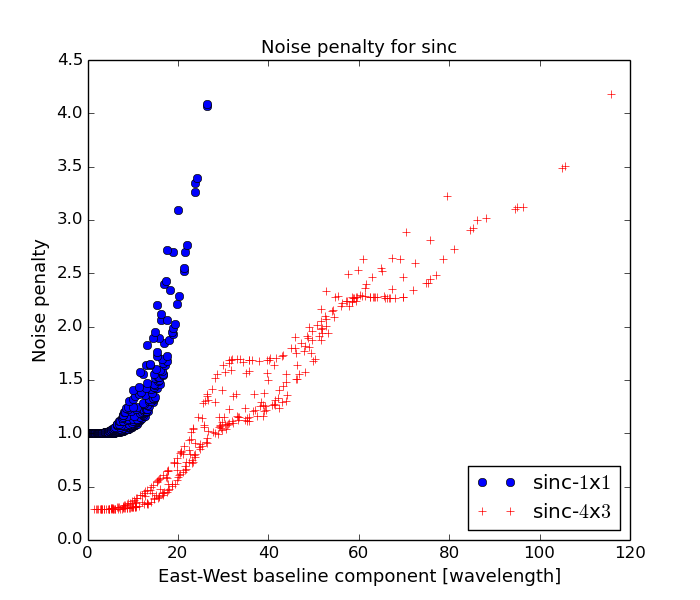
\includegraphics[width=.4\textwidth]{./Figures/per-baseline-noise-ratio-sinc.png}%
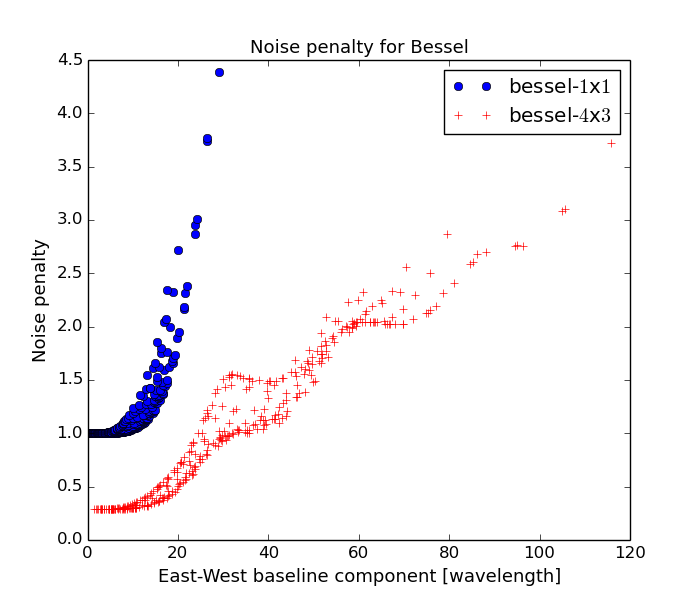
\includegraphics[width=.4\textwidth]{./Figures/per-baseline-noise-ratio-bessel.png}
\caption{Noise penalty w.r.t. normal averaging as a function of baseline length for two different BDWFs 
(sinc and Bessel), with and without overlap. JVLA-C, 1.4 GHz, sampling intervals of 100s and 
10 MHz. 
%\OMS{Marcellin, please check the numbers I gave are correct. Also please make the PDF figures the same size
%.}
}
\label{fig:per-baseline-noise}
\end{figure*}

\section{Simulations and results}

\newcommand{\BIN}[2]{#1s$\times$#2MHz}

In this section we use BDWFs to resample simulated visibility data, and study the effect on smearing and source 
suppression. Apart from a few examples documented separately, the basis interferometer configuration employed in 
the simulations corresponds to JVLA-C observing at 1.4 GHz. Similarly to Sect.~\ref{subsec:noise}, we create a 
``high-res'' measurement set corresponding to a 400s synthesis at 1s integration, with 30 MHz total bandwidth
centred on 1.4 GHz, divided into 360 channels of 83.4 kHz each.
%\OMS{Marcellin, check that I'm quoting correct numbers.}
The MS is populated by noise-free simulated visibilities corresponding to a single point source at 
a given distance from the phase centre. We then generate ``low-res'' MSs to receive the resampled visibilities,
resample the latter using a range of BDWFs, convert the visibilities to dirty images (using natural weighting
unless otherwise stated), and measure the peak source flux in each image. Since each dirty image corresponds to 
a single source, the peak flux gives us the degree of smearing associated with a given BWDF and sampling interval.

For the first set of simulations, the ``low-res'' MSs correspond to a 100s and 10MHz synthesis. We employ three 
sampling rates, \BIN{25}{2.5}, \BIN{50}{5} and \BIN{100}{10} (thus 4 timeslots and 4 channels, 2 timeslots
and 2 channels, and single-channel snapshot).

\begin{figure*}
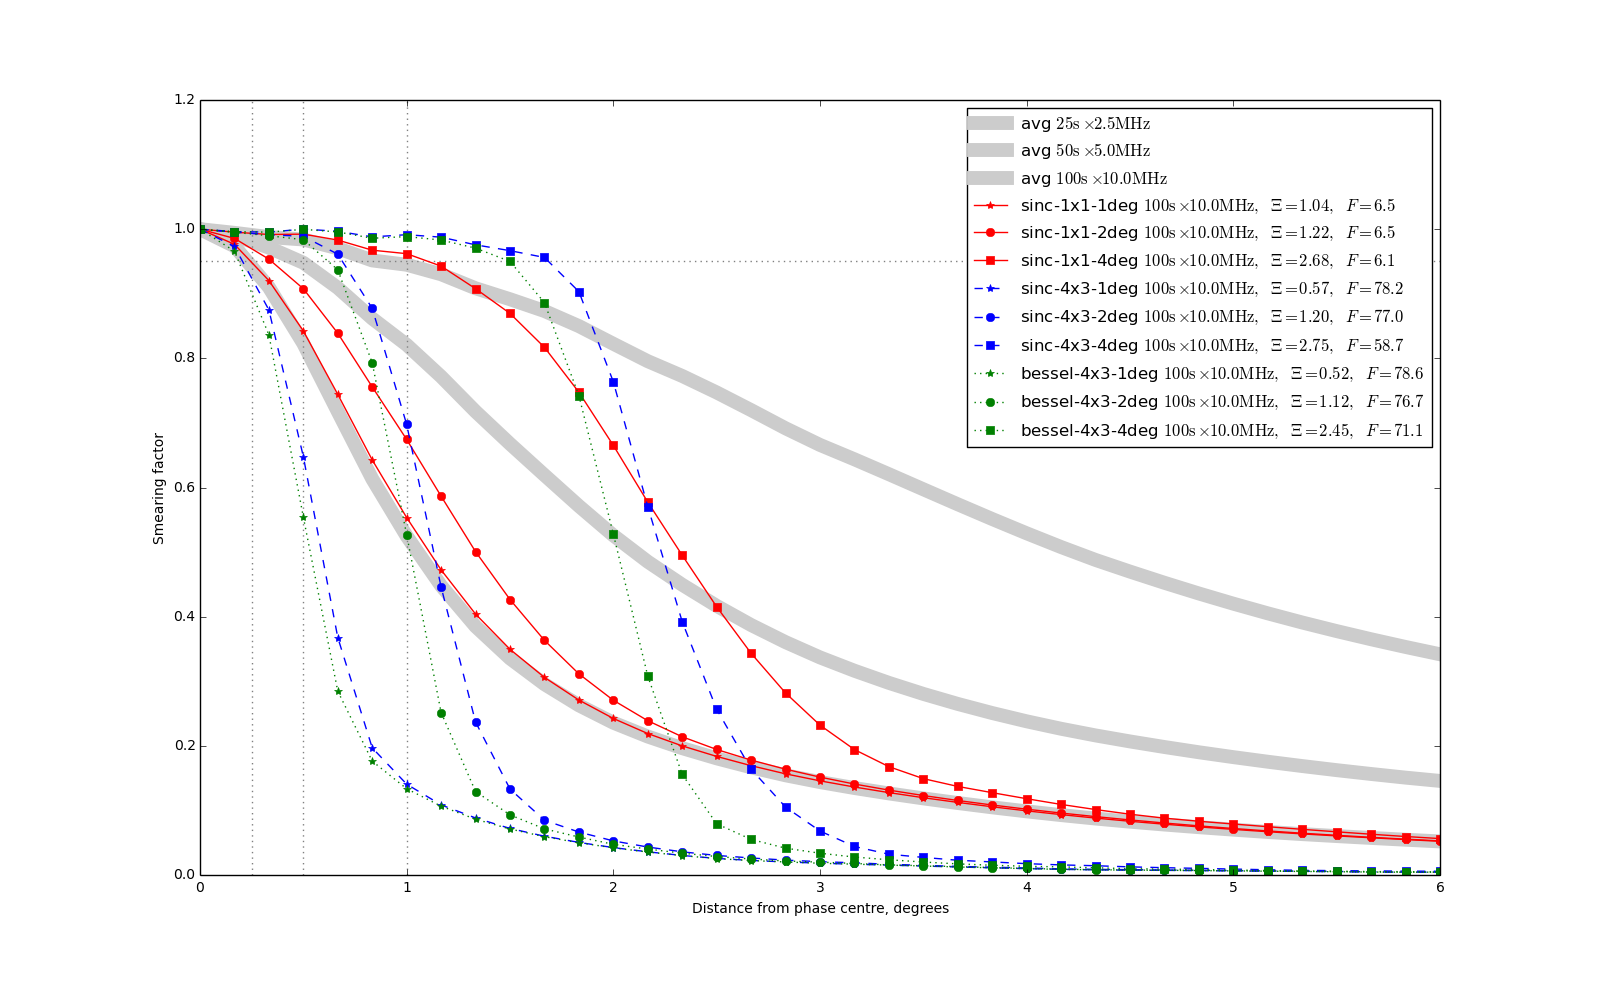
\includegraphics[width=.9\textwidth]{./Figures/suppression-10x100-3wfs.png}
\caption{JVLA-C 1.4 GHz. Smearing as a function of distance from phase centre, for conventional averaging with 
\BIN{25}{2.5}, \BIN{50}{5} and \BIN{100}{10} bins, and for several BDWFs with \BIN{100}{10} bins.
The noise penalty $\Xi$ and the far-source suppression factor $F$ are given relative to \BIN{25}{2.5}
averaging.}
\label{fig:results-example}
\end{figure*}
\begin{figure*}
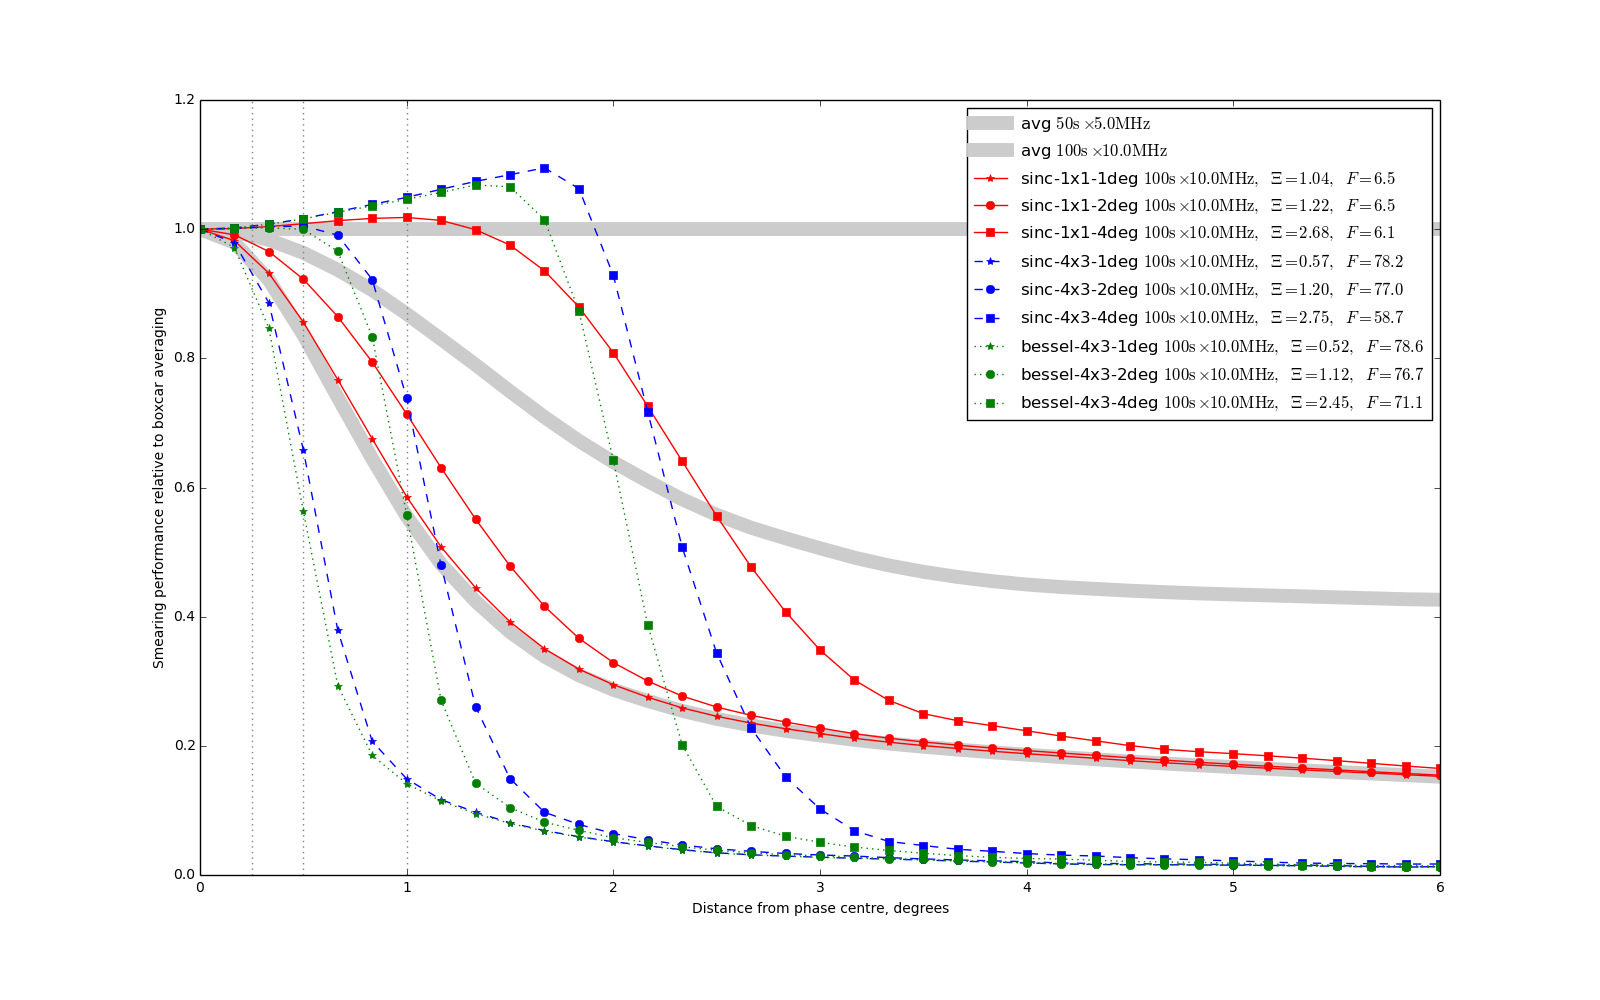
\includegraphics[width=.9\textwidth]{./Figures/relsuppression-10x100-3wfs.png}\\
\caption{JVLA-C 1.4 GHz. Results of Fig.~\ref{fig:results-example} normalized to the \BIN{25}{2.5} averaging curve.}
\label{fig:results-example2}
\end{figure*}

A typical performance comparison for the JVLA-C configuration at 1.4 GHz is given by Fig.~\ref{fig:results-example}.
This figure illustrates some of the principal achievements of the present work, so let us spend some time explaining it.
The horizontal axis represents distance from phase centre, while the vertical axis of the leff-hand plot represents  the
degree of smearing (left plot). Unity corresponds to no smearing; this is the case at phase centre, thus all curves
start at unity. The three thick grey curves correspond to normal averaging into \BIN{25}{2.5}, \BIN{50}{5} and
\BIN{100}{10}. We can (rather arbitrarily) define a series of ``acceptable'' smearing levels by specifying a  FoV
radius, and the maximum extent of smearing over that FoV. For the FoV radius, we may pick e.g. the half-power point  of
the PB, the main lobe of the PB, or extent of the first sidelobe of the PB. For JVLA's 25m dishes at this frequency,
these radius correspond to $\sim0.25^\circ$, $0.5^\circ$, and $1^\circ$, respectively; they are indicated by thin
vertical lines in the figure. The thin horizontal line indicates our chosen smearing threshold of $0.95$. In the right
plot,  all the curves are normalized with respect to the \BIN{25}{2.5} averaging curve.

For regular averaging, the three chosen bin sizes happen to roughly correspond to acceptable levels of smearing over the
three chosen FoV values. The other curves show the performance of a few different BDWFs, all at 100s$\times$10MHz
sampling. There are three types of BDWFs shown, indicated by line style (and colour, in the colour version of the plot):
\begin{description}
\item[\WF{sinc}{1}{1}] i.e. a non-overlapping sinc window (solid line, red)
\item[\WF{sinc}{4}{3}] i.e. an overlapping sinc window (dashed line, blue)
\item[\WF{bessel}{4}{3}] i.e. an overlapping Bessel window (dotted line, green)
\end{description}
These are tuned to three different FoV settings, as indicated by the plot symbol: $1^\circ$ (star), $2^\circ$ (circle),
$4^\circ$ (square). 

The plot is meant to show performance of BDWFs at \BIN{100}{10} versus a ``baseline case'' of \BIN{25}{2.5} averaging, 
the latter being an acceptable averaging setting for this particular frequency and telescope geometry. The legend 
next to the plot therefore indicates $\Xi$, the noise penalty associated with that particular BDWF, and $F$, the 
far source suppression factor. Both values are calculated w.r.t. the baseline case. Note the following salient features:

\begin{itemize}

\item All overlapping BDWFs provide outstanding far source suppression in this regime, with $F$ in the $60\sim80$ range. 
The non-overlapping sinc (solid red lines) only achieves $F~6$, which is similar to regular averaging
at the same rate. 

\item Noise performance is excellent for the $1^\circ$ BDWFs. There is a small noise penalty at $2^\circ$, and a larger 
(over a factor of 2) noise penalty at $4^\circ$. This can be easily understood by considering the shape of BDFWs as
a function of FoV: smaller FoVs correspond to broader windows that become more ``boxcar-like'' over the sampling
interval, and vice versa. This means that, in this particular configuration, BDWFs cannot achieve a FoV of $4^\circ$
at \BIN{10}{100} without a substantial sacrifice in sensitivity. We shall return to this issue below.

\item If the desired FoV size is $r\sim0.5-1^\circ$, overlapping BDWFs (sinc-4x3-2deg and bessel-
4x3-2deg) provide excellent performance at \BIN{100}{10}. Compared to averaging at \BIN{25}{2.5}, they achieve a factor
of 16 data compression with minimal loss of sensitivity, with excellent tapering behaviour: the smearing peformance 
across the FoV is equivalent to (or better) than that of normal averaging, and out-of-FoV source suppression is almost
two orders of magnitude higher.

\end{itemize}

Figure~\ref{fig:results-example2} presents the same results in an alternative way. Here, the recovered flux is shown 
relative to the baseline case of \BIN{25}{2.5} averaging. This clearly illustrates the excellent peformance of overlapping
BDWFs tuned to $2^\circ$.

\subsection{Noise penalties and overlapping BDWFs}

Values of $\Xi<1$ above may be paradoxical at first, since one can't theoretically exceed the noise performance of the
unweighted average. This, however, is an artefact of our short simulation. Overlapping BDWFs are essentially
averaging in ``bonus signal'' from regions of overlap extending outside the nominal time and frequency 
coverage. In our case, at \BIN{100}{10} sampling, a BDWF with $4\times3$ overlap is actually adding up signal over a
\BIN{400}{30} bin, i.e. a bin that is a factor of 12 larger (though of course the bonus sensitivity thus gained is much
less than the theoretically available $\sqrt{12}$, since the weights over the overlap regions correspond
to the ``wings'' of the WF, and are thus small). This can easily result in lower per-visibility noise than that 
achieved by regular averaging over \BIN{100}{10}, and correspondingly higher snapshot sensitivity.

In the more realistic case of a long, multiple-channel synthesis (what we'll call a \emph{full synthesis}), the
effects of bonus sensitivity disappear. While the noise on individual visibilities remains nominally lower in a full 
synthesis thanks to the overlap, it becomes correlated across neighbouring $uv$-bins, so there is no net gain 
in image-plane sensitivity. Strictly speaking, at the ``edge'' of the synthesis, overlapping BDWFs are still pulling 
in some bonus signal from overlap regions extending beyond the synthesis coverage, but since the area of this 
overlap is negligible compared to the coverage of the full synthesis, so is the effect of the bonus signal.

\begin{figure*}
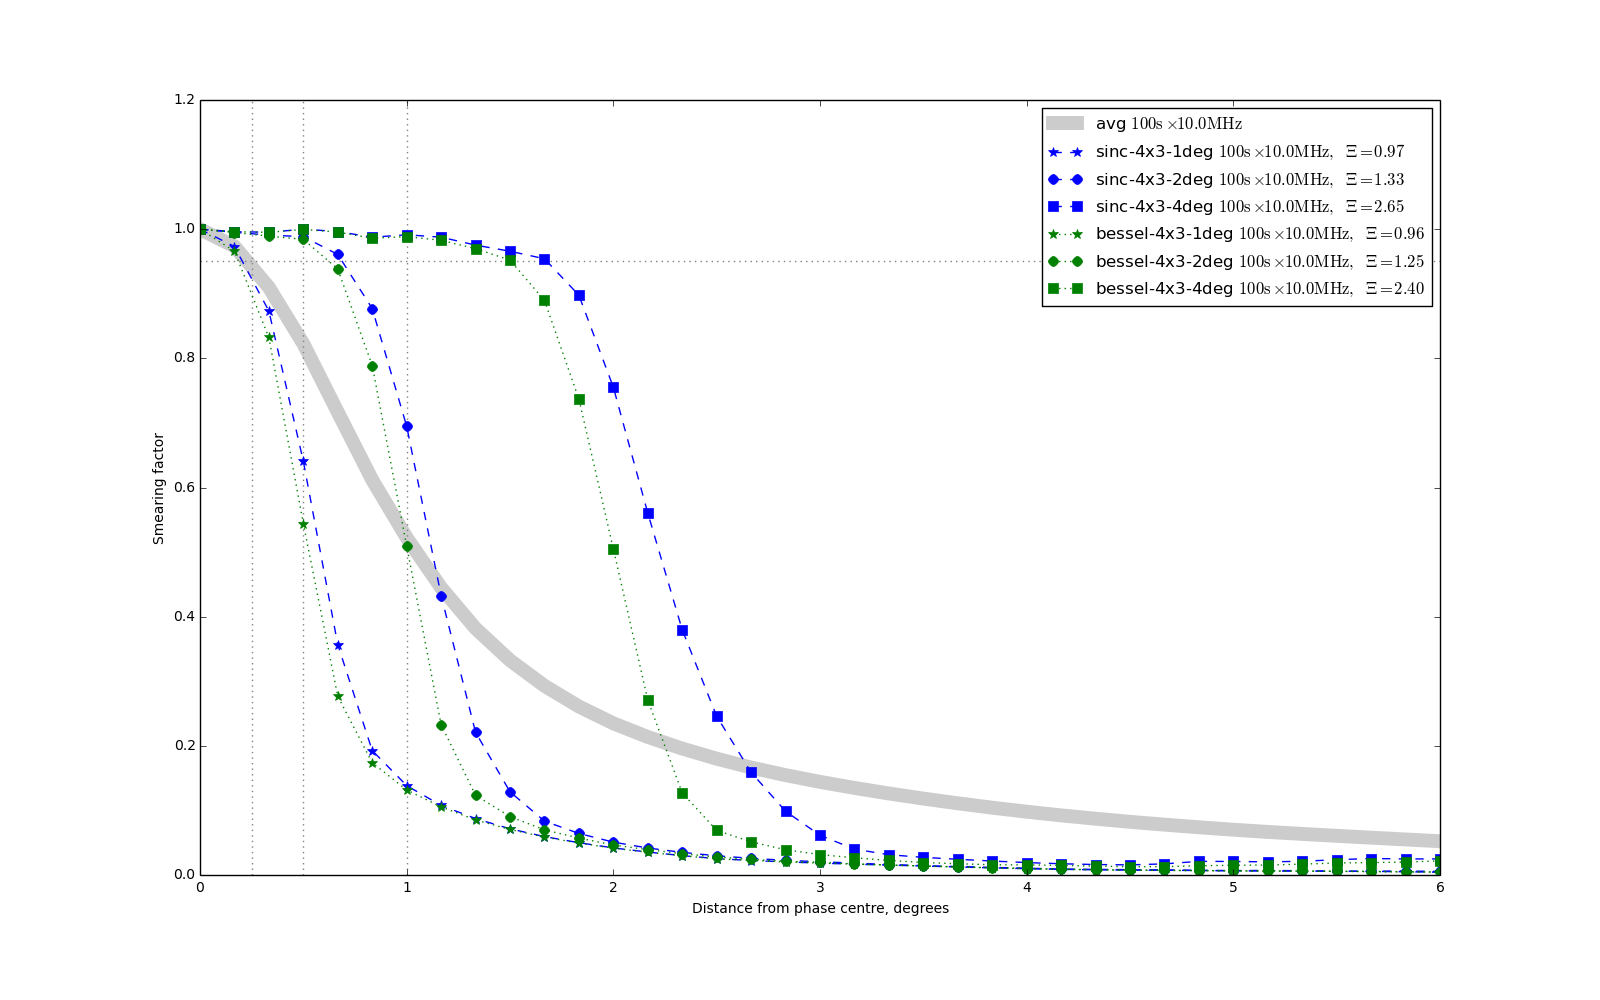
\includegraphics[width=.9\textwidth]{./Figures/suppression-longsynth.png}\\
\caption{JVLA-C 1.4 GHz, long wideband synthesis. Smearing as a function of distance from phase centre, 
for conventional averaging with \BIN{100}{10} bins, and for overlapping BDWFs with \BIN{100}{10} bins.
The noise penalty $\Xi$ is given relative to \BIN{100}{10} averaging.}
\label{fig:results-longsynth}
\end{figure*}

In other words, simulating a snapshot observation results in underestimated noise penalties, compared to the
real-life case of a full syntesis. We should expect the noise penalties to go up (and eventually exceed unity) as 
we increase the synthesis time and number of channels. Figure~\ref{fig:results-longsynth} presents the results of such 
a simulation. This shows a a \BIN{1800}{200} synthesis, sampled at the same rates as above. The results should be 
compared to and contrasted with those of Fig.~\ref{fig:results-example}. Note that the tapering response of BDWFs is 
nearly identical, while the noise penalties are indeed higher. With $4\times3$ overlap and \BIN{100}{10} sampling, 
the total signal accessed by overlapping BDWFs corresponds to \BIN{2100}{220}, which gives a theoretical maximum of 
a factor of $\sim1.13$ in bonus sensitivity. In other words, the values of $\Xi$ in Fig.~\ref{fig:results-longsynth}
are still underestimated, but by 13\% at most (which explains $\Xi<1$ for the $1^\circ$ case). From this we may safely
extrapolate that the noise penalty of BDWFs matched to $1-2^\circ$ FoVs will remain reasonable even for a much longer 
and wider band synthesis.

\subsection{FoVs and sampling rates}

For BDWFs, a given FoV tuning represents a characteristic scale in the $uv$-plane, which is inversely proportional to the 
FoV parameter. On the other hand, the $uv$-bin sampled by any given visibility is proportional to the integration time,
fractional bandwidth, and baseline length. Since the WF is truncated at edge of the averaging bin (which can be
larger by the sampling bin by a factor of several, if overlapping BDWFs are employed), there is, for any given baseline,
some kind of optimal range of $uv$-bin sizes over which BDWFs tuned to a particular FoV setting are ``efficient''. Over 
smaller bins, BDWFs become equivalent to a boxcar averaging, over larger bins, BDWFs penalize too much
sensitivity as they downweigh more samples. Since this optimal bin size is proportional to baseline length, the overall
optimum is dependent on the distribution of baselines in the array. 

Furthermore, the optimal sampling rate needs to be ``balanced'' in time and frequency for BDWFs to achieve optimal tapering
response. If the $uv$-bins are elongated, the WF becomes truncated (more boxcar-like) across the bin, which reduces its ability 
to induce the desired taper. Since the orientation of the bins changes as the baseline rotates, the 
cumulative effect is an average degradation of the tapering response, which becomes closer to that of boxcar averaging. In this sense,
the optimal $uv$-bin shape is square-like. This occurs when the fractional bandwidth is equal to the arc section swept
out by the baseline over one bin. For a polar observation (circular $uv$-tracks), we can express this as
\begin{equation}
\Delta \nu/\nu = 2 \pi (B_x/B)(\Delta t/24\mathrm{h}),
\end{equation}
where $B$ is the baseline length, and $B_x$ is its East-West component. Rewriting this in terms of more convenient units,
we end up with 
\begin{equation}
\frac{\Delta \nu_\mathrm{MHz}}{\Delta t_\mathrm{s}} \approx \frac{\nu_\mathrm{MHz}}{14000} \cdot \frac{B_x}{B},
\label{eq:optimal-binsize} 
\end{equation}
leading to a simple rule-of-thumb: at 1.4 GHz, an East-West baseline sweeps out a square-like bin when the 
integration time in seconds is 10 times the channel width in MHz (hence the use of bin sizes such as \BIN{100}{10} 
in the analysis here). 

\begin{figure*}
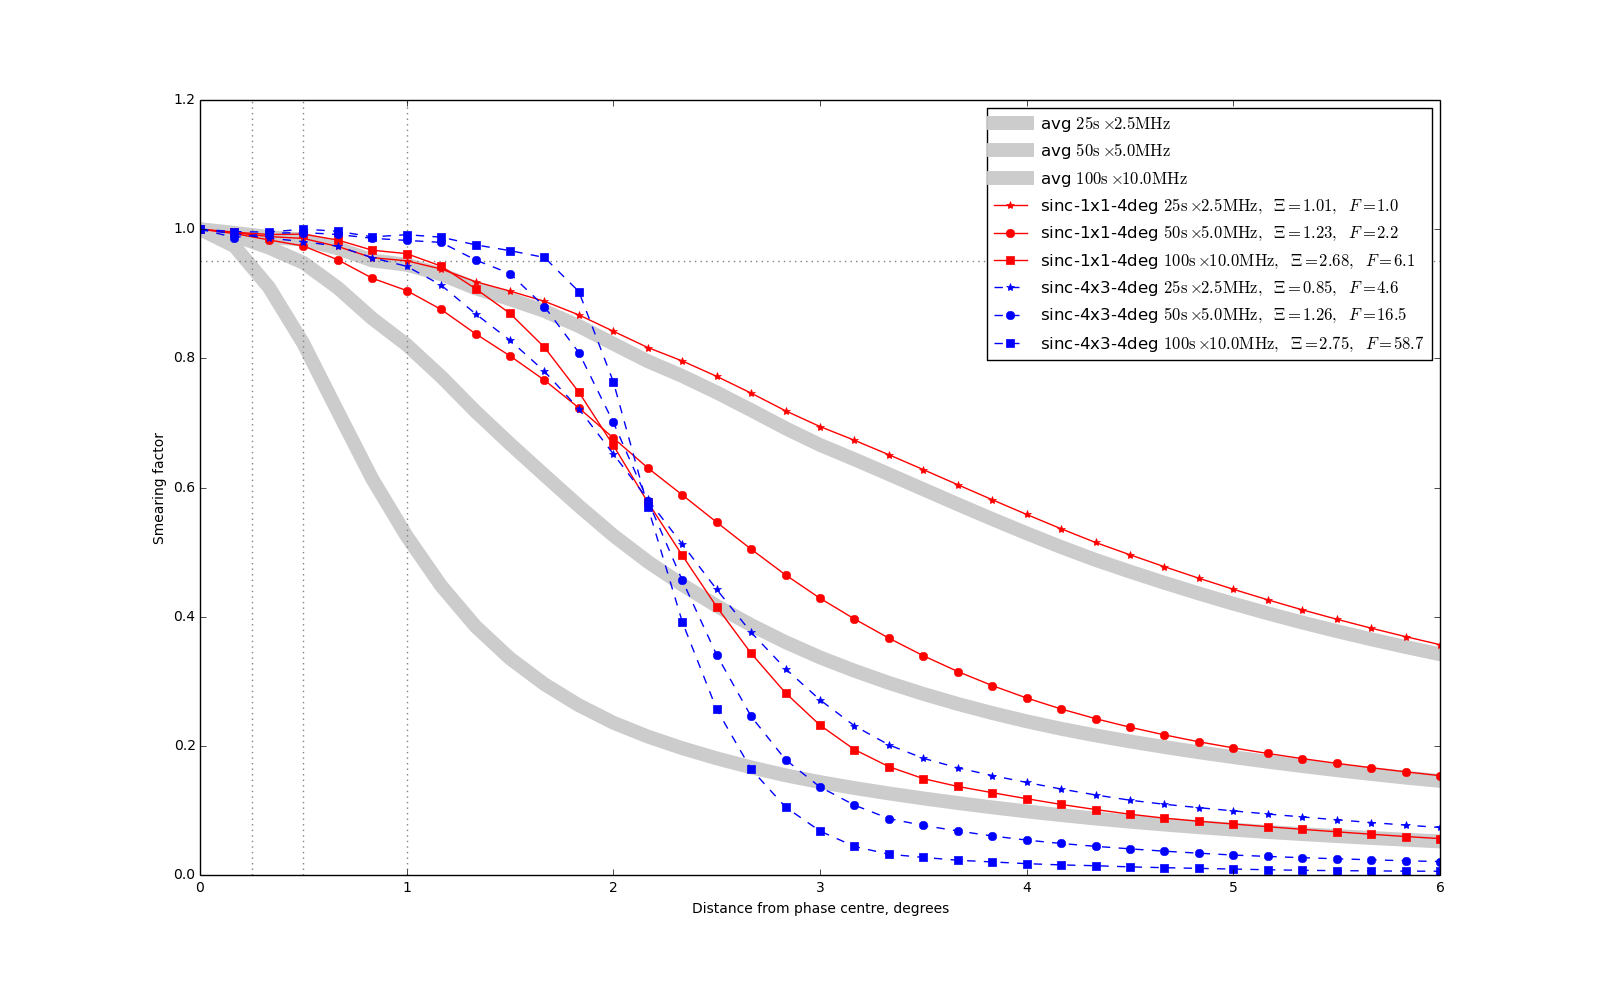
\includegraphics[width=.9\textwidth]{./Figures/suppression-25-100-sincs.png}
\caption{JVLA-C 1.4 GHz. Smearing as a function of distance from phase centre, for conventional averaging with 
\BIN{25}{2.5}, \BIN{50}{5} and \BIN{100}{10} bins, and for several BDWFs with \BIN{100}{10} bins.
The noise penalty $\Xi$ and the far-source suppression factor $F$ are given relative to \BIN{25}{2.5}
averaging.}
\label{fig:results-3sincs}
\end{figure*}
\begin{figure*}
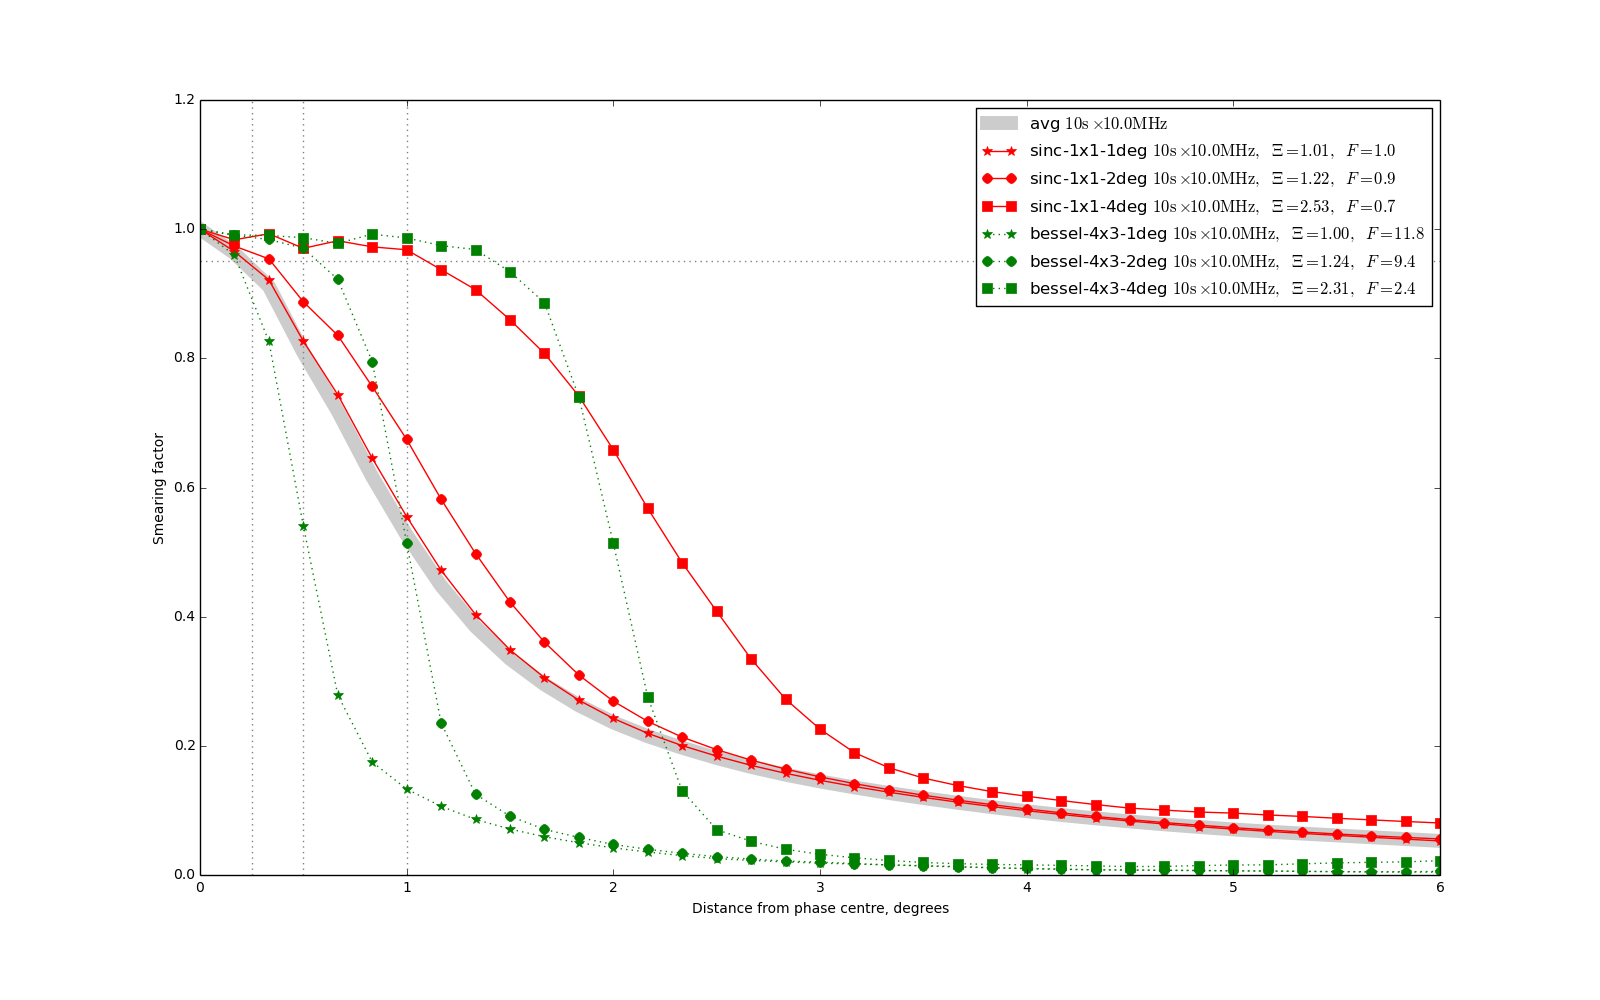
\includegraphics[width=.9\textwidth]{./Figures/suppression-14GHz.png}
\caption{JVLA-C 14 GHz. Smearing as a function of distance from phase centre, for conventional averaging with 
\BIN{2.5}{2.5}, \BIN{5}{5} and \BIN{10}{10} bins, and for several BDWFs with \BIN{10}{10} bins.
The noise penalty $\Xi$ and the far-source suppression factor $F$ are given relative to \BIN{2.5}{2.5}
averaging.}
\label{fig:results-14ghz}
\end{figure*}

The interaction between $uv$-bin size and tapering response is illustarted by Fig.~\ref{fig:results-3sincs}. Here we
compare the performance of two BDWFs tuned to a $4^\circ$ FoV -- a non-overlapping \WF{sinc}{1}{1} filter 
(solid red lines) and an overlapping \WF{sinc}{4}{3} filter (dashed blue lines) -- over three sampling bin sizes: 
\BIN{25}{2.5}, \BIN{50}{5} and \BIN{100}{10}. For reference, the performance of boxcar averaging over the same bin sizes
is indicated by the thick grey lines. Note how at the smaller bin size, the non-overlapping sinc is practically 
equivalent to a boxcar in terms of tapering response; at the larger bin size, it begins to shape the FoV. Introducing an 
overlap improves the response considerably. An overlapping filter at \BIN{25}{2.5} achieves almost the same tapering
response as a non-overlapping one at \BIN{100}{10} (which is not surprising, if one considers that the effective 
averaging bin size in the former case is \BIN{100}{7.5}). However, for all filters, at \BIN{100}{10} the noise penalty 
goes up quite sharply. 

This illustrates that \BIN{50}{5} is an appropriate BDWF sampling rate for achieving a $4^\circ$ FoV (for JVLA-C configuration at 
1.4 Ghz), providing a reasonable trade-off between tapering response and noise penalty. At higher sampling rates, 
the tapering response is degraded, while at lower sampling rates, the noise penalty increases. In comparison (as we 
saw in the previous section), for FoVs of $1-2^\circ$, BDWFs achieve a good trade-off at \BIN{100}{10} sampling.

It is interesting to consider how optimal BDWF sampling changes as a function of array size. Figure~\ref{fig:results-14ghz}
shows a simulation for JVLA-C at 14 GHz. (Since our results are completely determined by $uv$-plane geometry in 
wavelengths, this is equivalent to JVLA-C scaled up by a factor of 10 at an observing frequency of 1.4 GHz). 
From Eq.~\ref{eq:optimal-binsize}, we can see that square-like $uv$-bins correspond to 
sampling rate combinations such as \BIN{10}{10}. The simulation presented here is for a \BIN{1800}{200} synthesis,
i.e. is closer to the full synthesis rather than a snapshot case. Comparing Figs.~\ref{fig:results-14ghz} and 
\ref{fig:results-longsynth}, we find nearly identical BDWF performance (in terms of tapering response and
noise penalty) at 14 GHz and 1.4 GHz, with only the optimal sampling rate being different. 

\subsection{BDWFs for wide-field VLBI}

\begin{figure*}
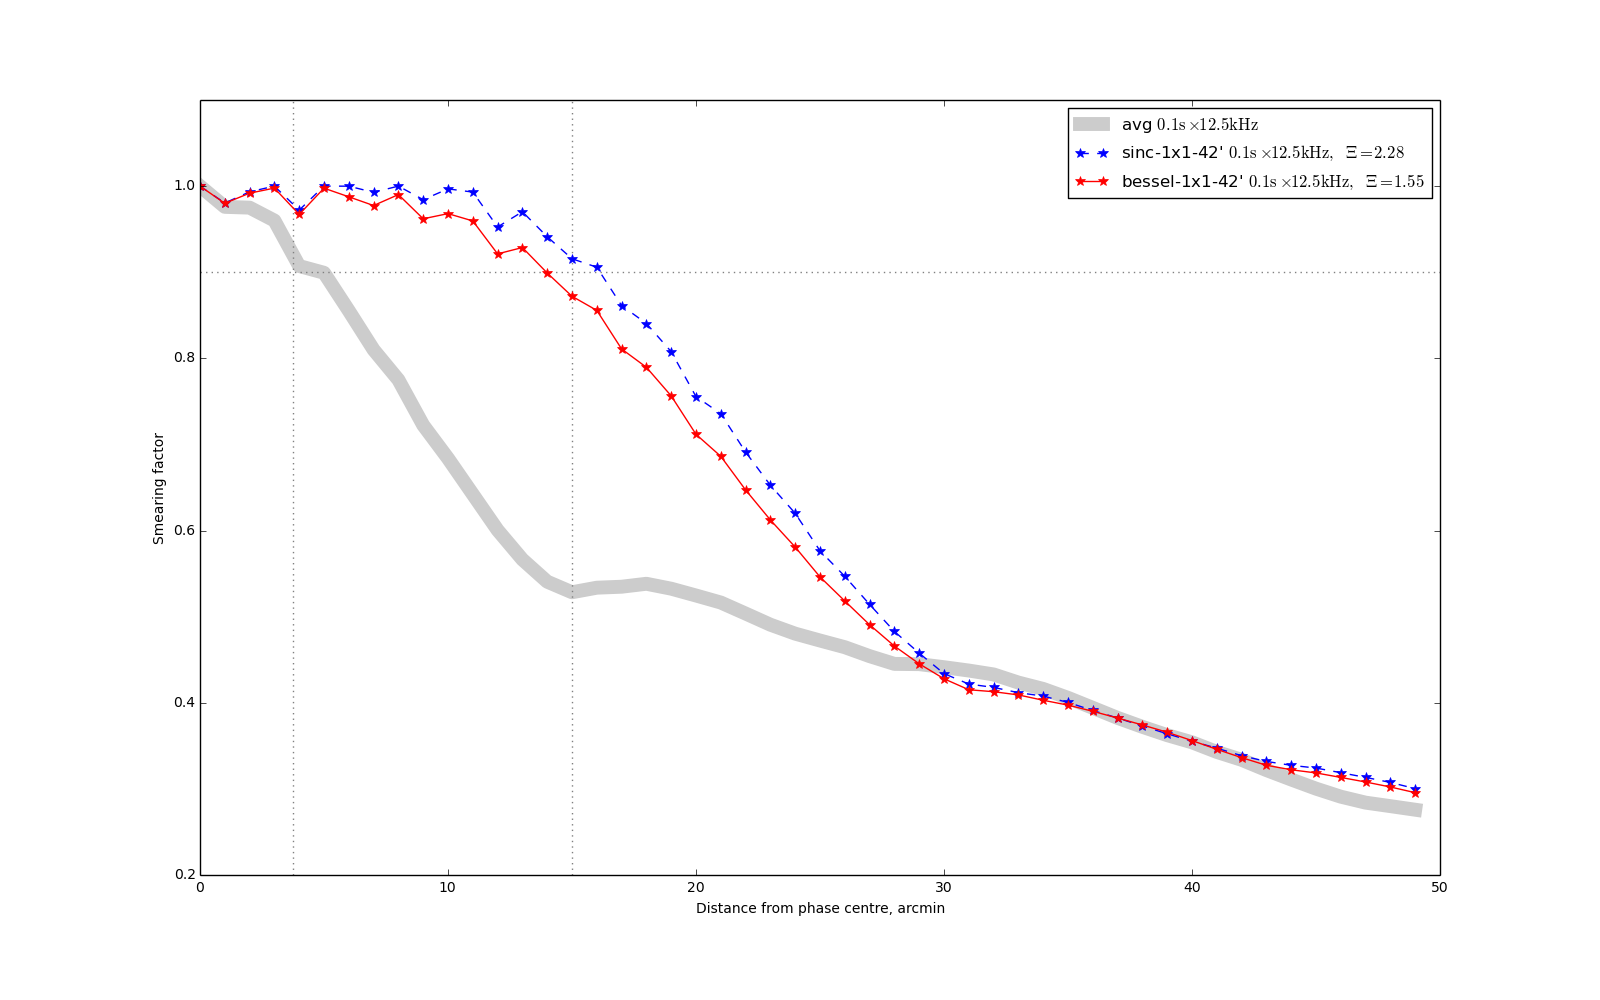
\includegraphics[width=.9\textwidth]{./Figures/suppression-vlbi.png}
\caption{VLBi simulation (10161km maximum baseline) at 1.6 GHz. Smearing as a function of distance from 
phase centre, for conventional averaging at 0.1s$\times$12.5kHz averaging, and for two BDWFs. The horizontal line
corresponds to 10\% smearing losses, the vertical lines are at $15'$ and $3'45''.$
}
\label{fig:results-vlbi}
\end{figure*}

In Fig.~\ref{fig:results-vlbi}, we investigate the performance of BDWFs in the regime of Very Long 
Baseline Interferometry (VLBI). Here, we simulate a 1.6 GHz VLBI observation employing eight stations 
(Effelsberg, Hartebeesthoek, Jodrell Bank, Noto, Onsala, Torun, JVLA, Westerbork, Shanghai), with a maximum baseline
of 10161km. With normal averaging in effect, the achievable FoV in VLBI is typically limited by smearing rather than the 
primary beam of any particular station. This has led to the development of techniques such as multiple-phase centre
VLBI, where a VLBI correlator produces multiple datasets per observation, corresponding to multiple phase centres 
within the same primary beam. 

As we can see from Fig.~\ref{fig:results-vlbi}, at a sampling rate of 0.1s$\times$12.5kHz, normal averaging
restricts the FoV to $\sim7.5'$. By contrast, both the sinc and Bessel BDWFs achieve a FoV of $~30'$ at the same 
sampling rate, with a relatively modest sensitivity penalty of 2.28 and 1.55, respectively. Effectively, this allows
the entire primary beam FoV to be mapped with a single VLBI dataset\footnote{Leaving aside the technical 
difficulties of actually imaging such a large FoV at VLBI resolutions.}. 

\section{Conclusions and future work}

The goal of this work was to demonstrate the application of baseline-dependent windowing functions to radio 
interferometry. We have demonstrated that BDWFs offer a number of interesting advantages over conventional averaging.
The first of these is data compression -- i.e. visibilities can be sampled at a lower rate, while retaining the primary 
beam FoV. Compression by a factor of 16 with relatively little loss of sensitivity has been demonstrated. The huge data 
rates from upcoming instruments such as ASKAP, MeerKAT and the future SKA1 mean that raw visibilities may need to be
discarded after calibration (unlike older instruments, where raw visibilities have typically been archived). This 
represents something of a risk to the science, as it precludes future improvements in calibration techniques from 
being later applied to the data. With BDWFs, at least a highly-compressed version of the visibilities may be retained.

The second potential benefit of BDWFs is the increased suppression of unwanted signal from out-of-FoV sources. This
reduces both the overall level of far sidelobe confusion noise, and lessens the impact of A-team sources in sidelobes.

Thirdly, BDWFs can have an interesting impact in the VLBI regime, as they allow the full primary beam FoV to be 
imaged using a single VLBI dataset. This opens the door to wide-field VLBI, which has herefore been impractical.

BDWFs have a number of potential downsides. The first one is a potential loss in sensitivity. Our simulations show 
that this can be kept within reasonable limits, especially if overlapping BDWFs are employed, and can be traded off with
compression rate. The second downside is an increase in computational complexity. Whether implemented in a correlator
or in post-processing, BDWFs (and especially overlapping BDWFs) require substantially more operations than simple averaging.
There may be other limits to the practical applicability of BDWFs. They are far less efficient if high spectral  
resolution is required, so their use may be limited to continuum observations. Furthermore, averaging over longer 
intervals requires accurate phase calibration, so high compression rates may only be achievable post-calibration.

An interesting avenue of future research is combining BDWFs with baseline-dependent averaging. As we saw above, the ability
of BDWFs to shape a FoV is somewhat limited by the fact that shorter baselines sweep out smaller bins in $uv$-space, with 
WFs over them becoming boxcar-like. If baseline-dependent averaging is employed, shorter baselines are averaged over
larger $uv$-bins, thus increasing the effect of BDWFs. 

Finally, we should note that the use of BDWFs results in a different position-dependent PSF than regular averaging (or
to put it another way, the smearing response of BDWFs results in a different smeared PSF shape). Future work will focus
on methods of deriving this PSF shape, with a view to incorporating this into current imaging algorithms.


\section*{Acknowledgements}

This work is based upon research supported by the South African Research Chairs Initiative of the Department of 
Science and Technology and National Research Foundation.


\bibliographystyle{mn2e}
\bibliography{m_paper}

% \appendix
% \section[]{Derivation of complex matrices}
% \label{app:complexmatrices}
% The complex matrices used in section \ref{sec:imaging} are explicitly derived in this appendix. In Eq.\ref{eqbb:linear}, the matrices
% $\mathbf{C}_{(t,\nu)}^{block}$ and $\mathbf{W}_{pq,(t,\nu)}^{block}$ are blocks diagonals  both of size $(4n_t n_{\nu})\times(4n_t 
% n_{\nu})$ explicitly expressed as follow:
% \begin{equation*}
% \mathbf{C}_{(t,\nu)}^{block}=
%   \begin{bmatrix}
%     \mathbf{c}_{(t,\nu)} & 0 & 0 & 0\\
%     0 &  \mathbf{c}_{(t,\nu)} &0 & 0 \\
%     0 & 0 & \mathbf{c}_{(t,\nu)} & 0\\
%       0 & 0 & 0 & \mathbf{c}_{(t,\nu)}\\
%   \end{bmatrix}
% \end{equation*}
% \begin{equation*}
% \mathbf{W}_{pq,(t,\nu)}^{block}=
%   \begin{bmatrix}
%     \mathbf{W}_{pq,(t,\nu)}& 0 & 0 & 0\\
%     0 &  \mathbf{W}_{pq,(t,\nu)} &0 & 0 \\
%     0 & 0 & \mathbf{W}_{pq,(t,\nu)} & 0\\
%       0 & 0 & 0 & \mathbf{W}_{pq,(t,\nu)}\\
%   \end{bmatrix}
% \end{equation*}
% In Eq.\ref{eq2:block}, the matrices $\mathbf{C}_{pq,(t,\nu)}^{block,n_{block}}$ and 
% $\mathbf{W}_{pq,(t,\nu)}^{block,n_{block}}$ are blocks diagonals both of size $(4N_v^{pq}n_t n_{\nu})\times (4N_v^{pq}n_t n_{\nu})$, and 
% the sampled visibilities $\mathbf{V}_{pq,(t,\nu)}^{samp,nblock}$ is a one row matrix of size $(N_v^{pq}4 n_t n_{\nu})\times (4 n_t 
% n_{\nu})$ 
% made of $\textbf{V}_{pq,(t,\nu)}^{samp}$. These matrices are explicitly expressed as follow:
% \begin{equation*}
% \mathbf{C}_{pq,(t,\nu)}^{block,n_{block}}=
%   \begin{bmatrix}
%     \mathbf{C}_{pq,(t,\nu)}^{block} &\dots & 0 & \dots & 0\\
%     \vdots & \vdots & \vdots & \vdots & \vdots\\
%     0 & \dots& \mathbf{C}_{pq,(t,\nu)}^{block} &\dots & 0\\
%     \vdots & \vdots & \vdots & \vdots & \vdots \\
%     0 & \dots& 0 &\dots & \mathbf{C}_{pq,(t,\nu)}^{block}\\
%   \end{bmatrix}
% \end{equation*}
% \begin{equation*}
% \mathbf{W}_{pq,(t,\nu)}^{block,n_{block}}=
%   \begin{bmatrix}
%     \mathbf{W}_{pq,(t,\nu)}^{block} &\dots & 0 & \dots & 0\\
%     \vdots & \vdots & \vdots & \vdots & \vdots\\
%     0 & \dots& \mathbf{W}_{pq,(t,\nu)}^{block} &\dots & 0\\
%     \vdots & \vdots & \vdots & \vdots & \vdots \\
%     0 & \dots& 0 &\dots & \mathbf{W}_{pq,(t,\nu)}^{block}\\
%   \end{bmatrix}
% \end{equation*}
% \begin{eqnarray*}
% \mathbf{V}_{pq,(t,\nu)}^{samp,n_{block}}&=&\Big(\mathbf{V}_{pq,(t,\nu)}^{samp,1},\dots, \mathbf{V}_{pq,(t,\nu)}^{samp,k}, \dots,
% \mathbf{V}_{pq,(t,\nu)}^{samp,N^{pq}_v}\Big)^{\dagger}. 
% \end{eqnarray*}
% In Eq.\ref{eq:noise}, the matrix $\mathbf{B}$ of size $(N_v 4 n_t n_{\nu})\times (4 n_t n_{\nu})$ is defined as follow:
% \begin{equation*}
% \mathbf{B}_{}=
%   \begin{bmatrix}
%     \mathbf{C}_{01,(t,\nu)}^{block,n_{block}}\cdot \mathbf{W}_{01,(t,\nu)}^{block,n_{block}}\\
%     \vdots\\
%     \mathbf{C}_{ik,(t,\nu)}^{block,n_{block}}\cdot \mathbf{W}_{ik,(t,\nu)}^{block,n_{block}}\\
%     \vdots \\
%     \mathbf{C}_{jl,(t,\nu)}^{block,n_{block}}\cdot \mathbf{W}_{jl,(t,\nu)}^{block,n_{block}}
%   \end{bmatrix}
% \end{equation*}
% % \section[]{Sky tapering function with averaging}
% % \label{label:similarimaging}
% % The measured sky intensity of the array is derived from the inverse Fourier transform of the sum of the sample visibilities 
% % measured at each baseline.
% % \begin{eqnarray*}
% %  \mathcal{I}^{D}_{l,m}&=& \mathcal{F}^{-1}\Bigg\{\sum_{pq} c_{pq,(t,\nu)}\cdot\Big(\Pi_{pq}\circ V_{pq}^{samp}\Big)_{(t,\nu)}\Bigg\}\\
% % 		      &=&\sum_{pq} \mathcal{F}^{-1}\{c_{pq,(t,\nu)}\}\circ \Big(\mathcal{F}^{-1}\{\Pi_{pq,(t,\nu)}\}\cdot 
% % \mathcal{F}^{-1}\{V_{pq,(t,\nu)}^{samp}\}\Big)
% % \end{eqnarray*}
% % \begin{eqnarray*}	     
% % \mathcal{I}^{D}_{l,m}&=&\sum_{pq}\mathcal{F}^{-1}\{\Pi_{pq,(t,\nu)}\}\cdot\bigg(\mathcal{F}^{-1}\{S_{pq}\cdot V_{pq,(t,\nu)}\}
% % \bigg)
% % \end{eqnarray*}
% % recall from section \ref{sec:AvgCon} that $S_{pq}$ is the sampling function of the baseline $pq$ and $\Pi_{pq,(t,\nu)}$ is the 
% % boxcar window.  This can be re-written as
% % \begin{eqnarray*}	     
% % \mathcal{I}^{D}_{l,m}&=&\sum_{pq} \mathcal{R}_{pq} \cdot\bigg(\mathcal{B}_{pq}\circ \mathcal{I}^{sky}_{l,m}\bigg)
% % \end{eqnarray*}
% % If all baselines are seen the same sky, then we can write:
% % \begin{eqnarray*}	     
% % \mathcal{I}^{D}_{l,m}&=&\mathcal{R}_{}\cdot\Bigg(\bigg(\sum_{pq}\mathcal{B}_{pq}\bigg)\circ \mathcal{I}^{sky}_{l,m}\Bigg)
% % \end{eqnarray*}
% % Here, $\mathcal{B}_{pq}$ is the point spread function for the baseline $pq$ and $\mathcal{R}_{pq}= \mathcal{R}$ is the sky taper, where 
% % $\mathcal{R}_{}=sinc$.\\
% % \\
\bsp
\label{lastpage}
\end{document}
